\documentclass[12pt,twoside,a4paper]{article}
\usepackage[utf8]{inputenc}
\usepackage[english]{babel}

\usepackage{float}

\usepackage{url}

\usepackage{caption}
\usepackage{subcaption}

\usepackage{graphicx}
\graphicspath{{./images/}}

\usepackage[authoryear,square]{natbib}
\bibliographystyle{dinat}

\newcommand{\papertitle}{Observations on Almost OU Tangles}
\newcommand{\paperauthor}{Albert \v Silvans}

%\usepackage[a4paper]{geometry}
\usepackage[a4paper,width=150mm,top=25mm,bottom=25mm,bindingoffset=6mm]{geometry}


\usepackage{multirow}

\usepackage{fancyhdr}
\pagestyle{fancy}
\fancyhead[LE,RO]{}
\fancyhead[LO,RE]{\rightmark}
\fancyfoot{}
\fancyfoot[LO, RE] {\thepage}

\title{\papertitle}
\author{\paperauthor}
\date{\today}

\usepackage{amsthm}
\usepackage{amsmath}
\usepackage{amsfonts}
\usepackage{amssymb}
\renewcommand{\qedsymbol}{$\blacksquare$}

\usepackage{cleveref}
\usepackage{enumitem}

\theoremstyle{definition}
\newtheorem{theorem}{Theorem}
\newtheorem{corollary}{Corollary}
\newtheorem{definition}{Definition}

\usepackage{pdfpages}

\begin{document}


\includepdf{bachelor-project-front-page-thesis.pdf}
\null\thispagestyle{empty}\newpage
\tableofcontents 				\newpage
\section{Introduction}

In the article \citep{barnatan2020tangles} we are introduced with some Knot Theoretic structures including tangles, tangle diagrams, braids, most importantly the Over then Under form of a tangle, or OU form for short, followed by a proposed algorithm for bringing a tangle diagram into an OU form, and some results relating to this form.

Although the results presented in the previously mentioned article are quite broad and general, in our article for the sake of simplicity we restrict ourselves to the special case of a tangle with a single strand, and focus on what properties or patterns we can discover by examining 1-tangles under the process of the OU form algorithm. We shall see that our choice of tangles to study will prove to be erroneous, and that we will encounter a level of complexity that we did not bargain for. Specifically, the only tangle diagrams that behave nicely under the algorithm are trivial, and even then there is a set of trivial diagrams which do not behave nicely. Furthermore the algorithm in the case of misbehavior never terminates, and the diagrams that are produced at each iteration slowly tend to the realm of the wild. 

Given the level of research intended here, before we begin we must draw out the definitions and concepts necessary to understand, reason, and ask further questions about this topic. We settle with a working definition, and attempt to introduce only the bare minimum. Should the reader be interested in a more comprehensive overview of Knot Theory, they are directed to the works \citep{adams_1994} and \citep{lickorish_1997}.

  		\newpage
\section{Tangles}

\subsection{Tangle diagrams}

Intuitively a tangle diagram is just that: a diagram. One finds a clear area on their paper, draws some lines with some over and under strands in mind. Typically an under strand is denoted by a break in the strand where the crossing should be, we see an example of a tangle diagram in \Cref{fig:tangle_diagram}.

\begin{definition}\textbf{(Tangle diagrams)}
Consider some closed, bounded, convex subset $B\subset\mathbb R^2$, and $n\in\mathbb N$ pairs of points $(a_n,b_n)$ on the boundary of $B$ with $a_i\neq a_j$ and $a_i\neq b_j$ for all $1\le i,j\le n$. Define for each $1\le i\le n$ a map $\phi_i:[0,1]\to B$ such that:
\begin{enumerate}
\item $\phi_i(0)=a_i$, $\phi_i(1)=b_i$, an orientation on the diagram is induced by the orientations of the $\phi_i$,
\item $\phi_i((0,1))\subset B$, i.e the image of $(0,1)$ is fully contained in $B$, we call $\phi_i((0,1))\subset B$ a \textit{strand},
\item We call $c\in B$ a \textit{crossing} if $c$ is in the image of 2 maps $\phi_i$,$\phi_j$, where if $i\neq j$ their preimages $\phi_i^{-1}(c),\phi_j^{-1}(c)$ have only one point, and if $i=j$, then the preimage of $c$ has 2 points. If a point is not a crossing, then it is in the image of at most one map, and its preimage contains a single point,
\item for each crossing $c$ take a neighborhood that contains no other crossing, in the neighborhood designate one \textit{over}, and one \textit{under} strand.
\end{enumerate}
We call this construction an \textit{n-Tangle Diagram}
\end{definition}

\begin{figure}[h!]
\centering
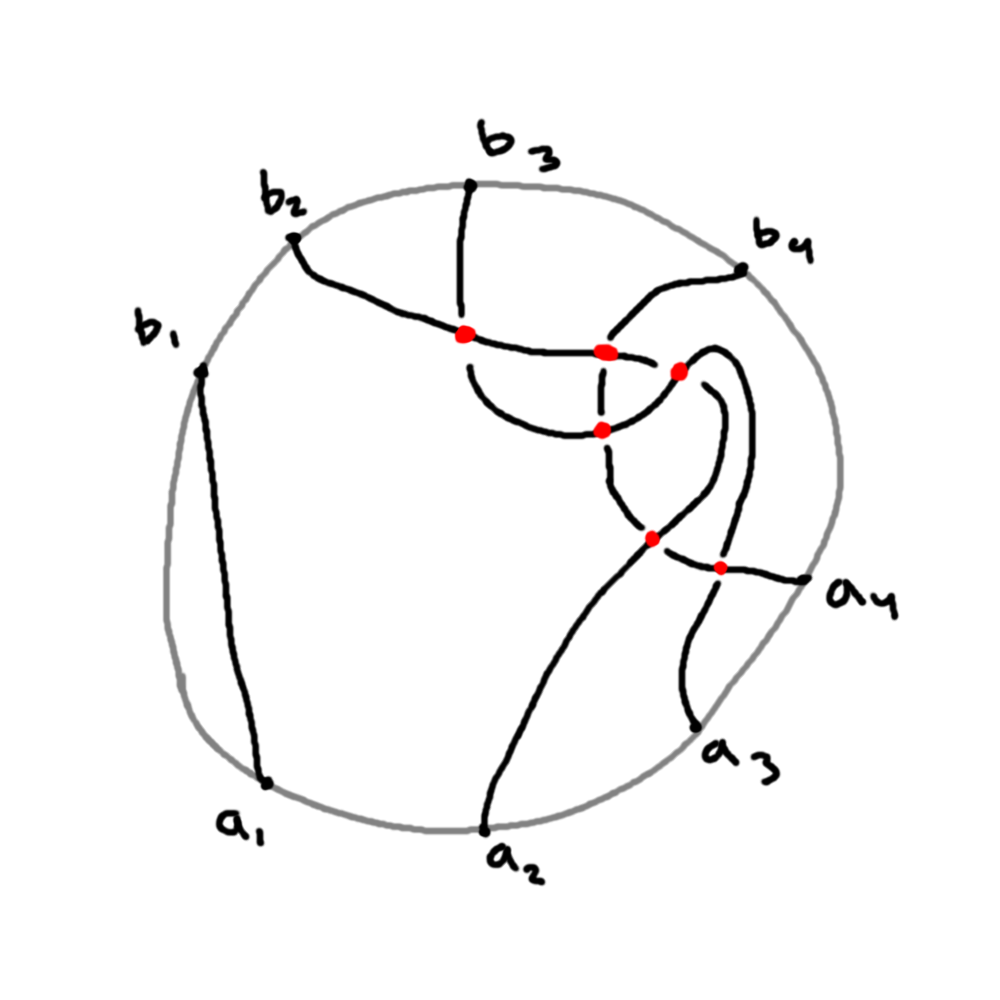
\includegraphics[width=0.4\textwidth]{tangle_diagram.png}
\caption{An example of a tangle diagram, notice there are 8 labeled points on the boundary (in grey) and each crossing (in red) is produced by at most two strands.}
\label{fig:tangle_diagram}
\end{figure}

The above definition is quite technical for the sake of clarity in how to generate a tangle diagram. In further discussions we will not use this level of precision, and simply focus on the combinatorial information of tangle diagrams, i.e. the relative position and orientation of the crossings. With regard to this combinatorial aspect there are maps or ``moves" that relate equivalent diagrams, those being the Reidermeister moves.


\subsection{Reidermeister moves, Tangles, the Tame and Wild}

\begin{definition}\textbf{(Reidermeister moves/ Isotopies)}
A region of a tangle diagram containing a configuration of strands and crossings as indicated in \Cref{fig:Rmoves} may be replaced by the associated configuration to produce a new tangle diagram. The new tangle diagram is equivalent to the old by a Reidermeister move.
\begin{figure}[h!]
\centering
\begin{subfigure}{0.31\textwidth}
\centering
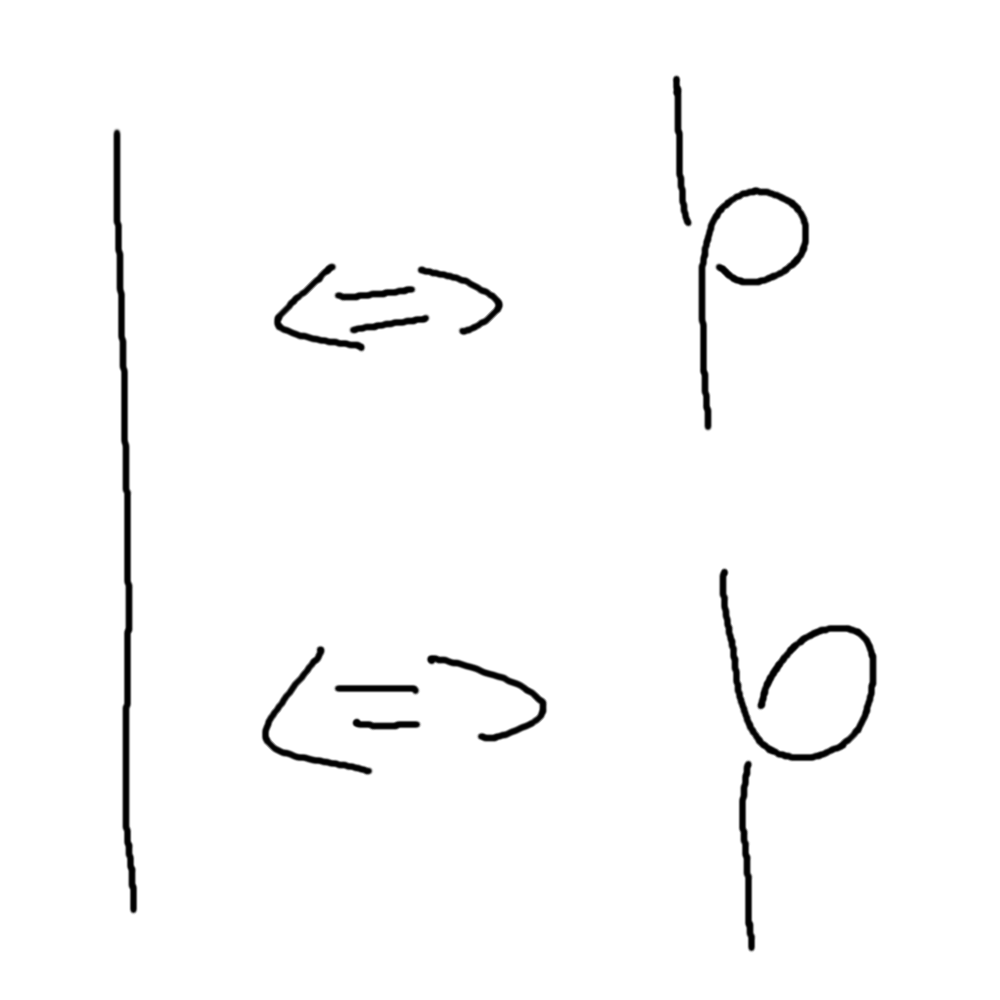
\includegraphics[width=\textwidth]{R1move.png}
\caption{The first move}
\label{fig:R1move}
\end{subfigure}
\hfill
\begin{subfigure}{0.31\textwidth}
\centering
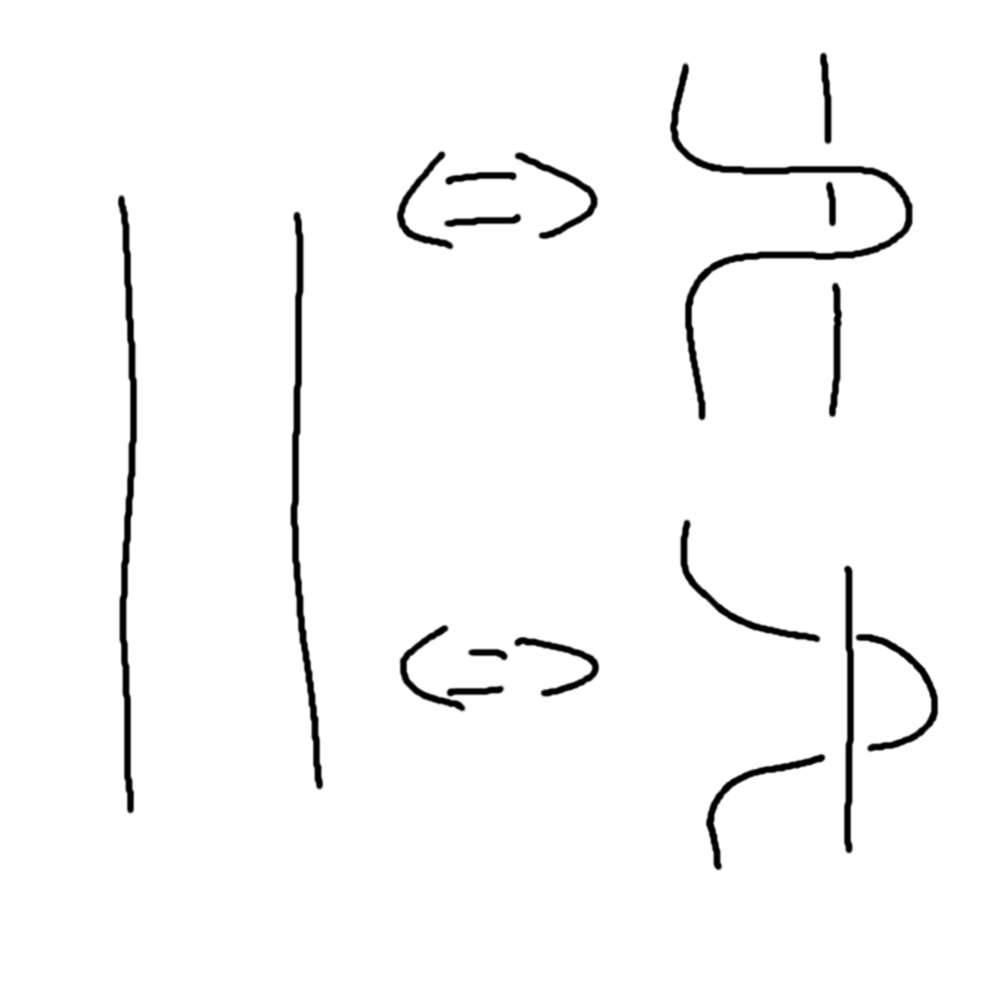
\includegraphics[width=\textwidth]{R2move.png}
\caption{The second move}
\label{fig:R2move}
\end{subfigure}
\hfill
\begin{subfigure}{0.31\textwidth}
\centering
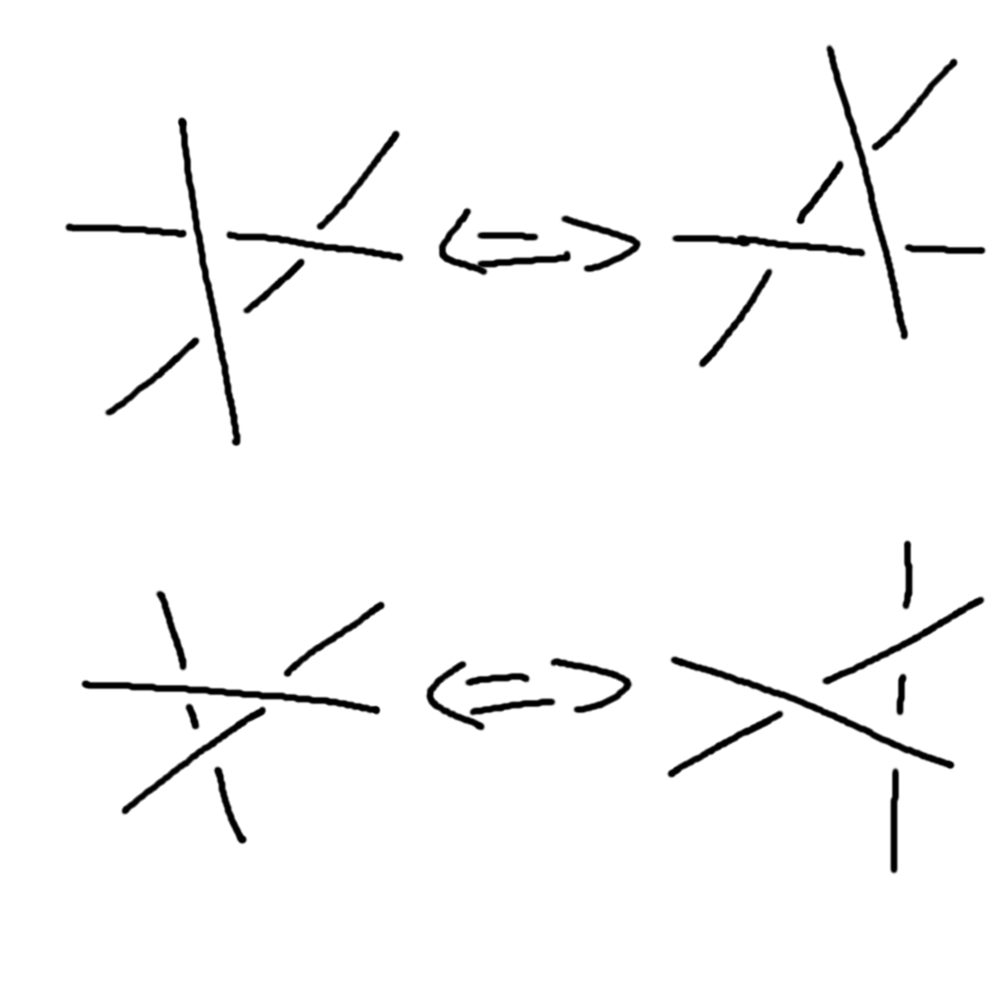
\includegraphics[width=\textwidth]{R3move.png}
\caption{The third move}
\label{fig:R3move}
\end{subfigure}
\caption{The 3 basic Reidermeister moves}
\label{fig:Rmoves}
\end{figure}
\end{definition}
The Reidermeister moves define an equivalence relation of tangle diagrams, which then defines an eqiuvalence class of tangle diagrams which we call a \textit{Tangle}. If we were to imagine tangle diagrams as tangible strands like shoelaces, and were to perform a sequence of Reidermeister moves, then intuitively we see that we either complicate or simplify the diagram but if were to take the ends of the laces and pull, ignoring friction, we get the same shape no matter what Reidermeister moves we apply.

\begin{definition}
A Tangle is an equivalence class of tangle diagrams under the relation of Reidermeister moves.
\end{definition}
Lastly we need to make a distinction between two varieties of tangle diagrams that our definition permits. Typically, when working with tangle diagrams we assume that the strands are either smooth or that they are homeomorphic to a finite polygonal chain, i.e. the strands are made from finitely many line segments, that way we can avoid pathological situations that are hard to understand, with this in mind we make this distinction a definition 

\begin{definition}
A tangle the strands of which are homeomorphic to a finite polygonal chain is called a \textit{Tame Tangle}. A tangle that is not tame is a \textit{Wild Tangle}.
\end{definition}

One might wonder why this condition was not included into the definition of a tangle diagram, and it will become clear once we discuss the algorithm in the next subsection. Before this we must mention orientations on diagrams and OU tangle diagrams.

\subsection{Oriented Gauss notation, OU diagrams}

As mentioned before we focus on the combinatorial information of a tangle diagram, so we ignore the parametrizations of each strand, and only care about the crossings and how they appear on the strands. We may abstract our diagrams to hold only this information, to do so we chose the Oriented Gauss notation or Oriented Gauss code. To produce the Oriented Gauss code we follow the steps:

\begin{enumerate}
\item Prescribe an order to the strands
\item For each strand prescribe an orientation, this is typically given by the map $\phi_i$ associated to the strand in question,
\item For each crossing assign a name, typically a unique integer, and a sign either $+$ or $-$ taking into account the orientations of the strands as shown in \Cref{fig:crossing},
\item For each strand associate a string of symbols by following from the start point to the end point and for each crossing we encounter we record either the symbol $O^s_i$ or $U^s_i$ where $O$ for over if our current strand is over, $U$ for under, $s$ for the sign of the crossing, and $i$ the name of the crossing encountered.
\item The ordered set of the previously recorded strings is called the Oriented Gauss code.
\end{enumerate}

\begin{figure}[h!]
\centering
\begin{subfigure}{0.20\textwidth}
\centering
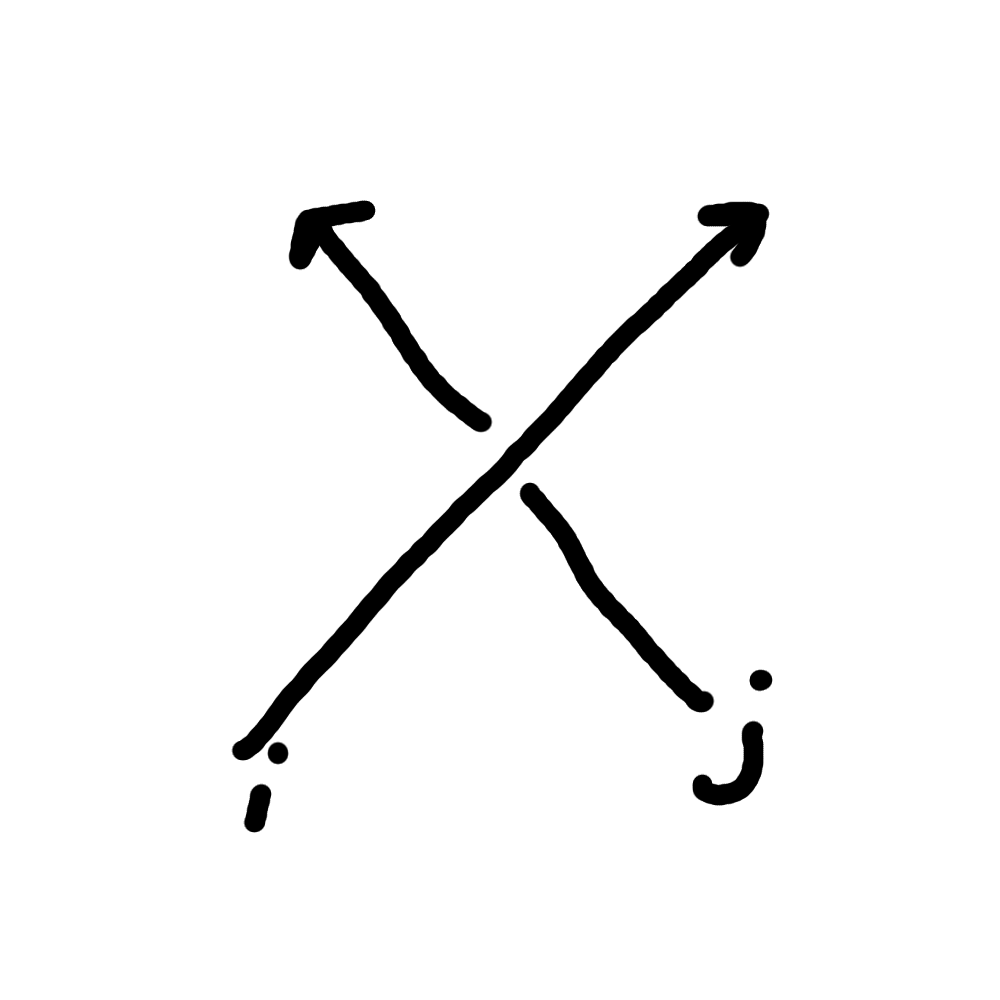
\includegraphics[width=\textwidth]{crossing+1.png}
\caption{This crossing is assigned +}
\label{fig:crossing:+1}
\end{subfigure}
\hspace{1cm}
\begin{subfigure}{0.20\textwidth}
\centering
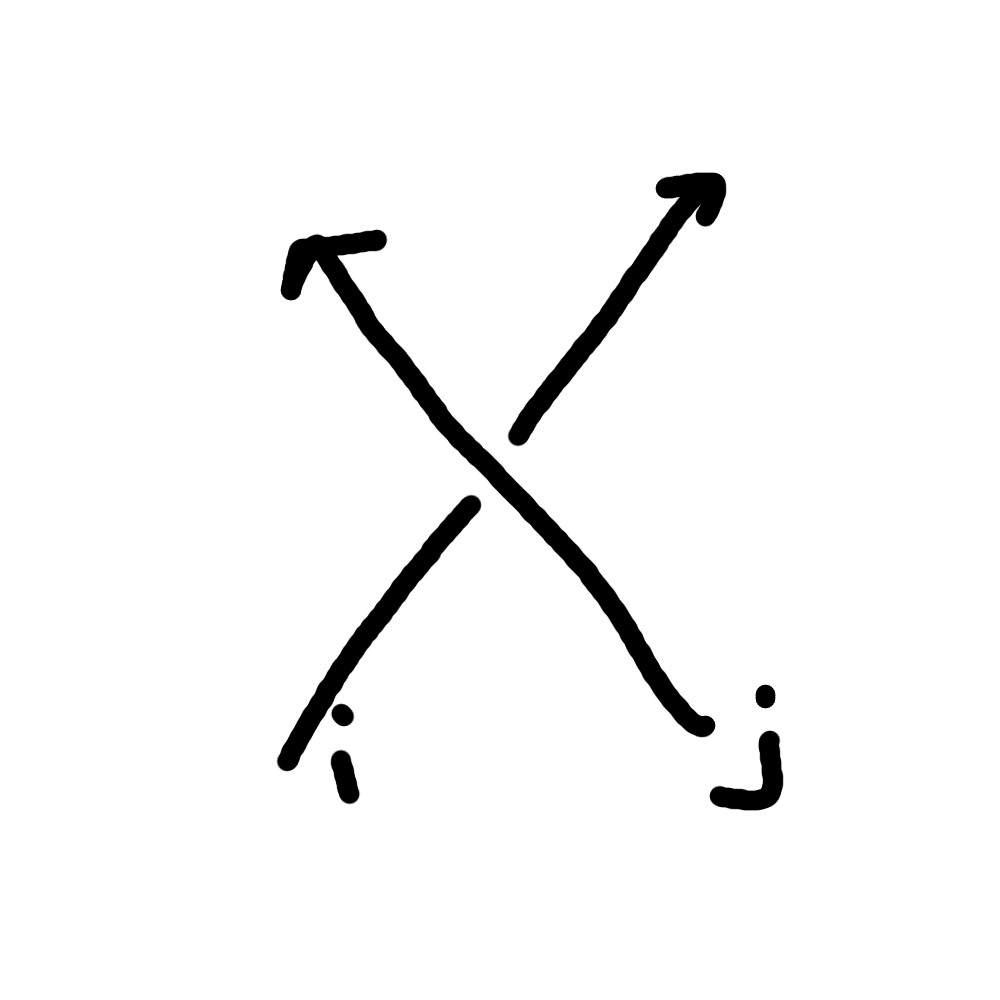
\includegraphics[width=\textwidth]{crossing-1.png}
\caption{This crossing is assigned -}
\label{fig:crossing:-1}
\end{subfigure}
\caption{Types of crossings by orientation.}
\label{fig:crossing}
\end{figure}

We provide some examples of tangles and their Oriented Gauss codes in \Cref{fig:Gaussexamples}

\begin{figure}[h!]
\centering
\begin{subfigure}{0.31\textwidth}
\centering
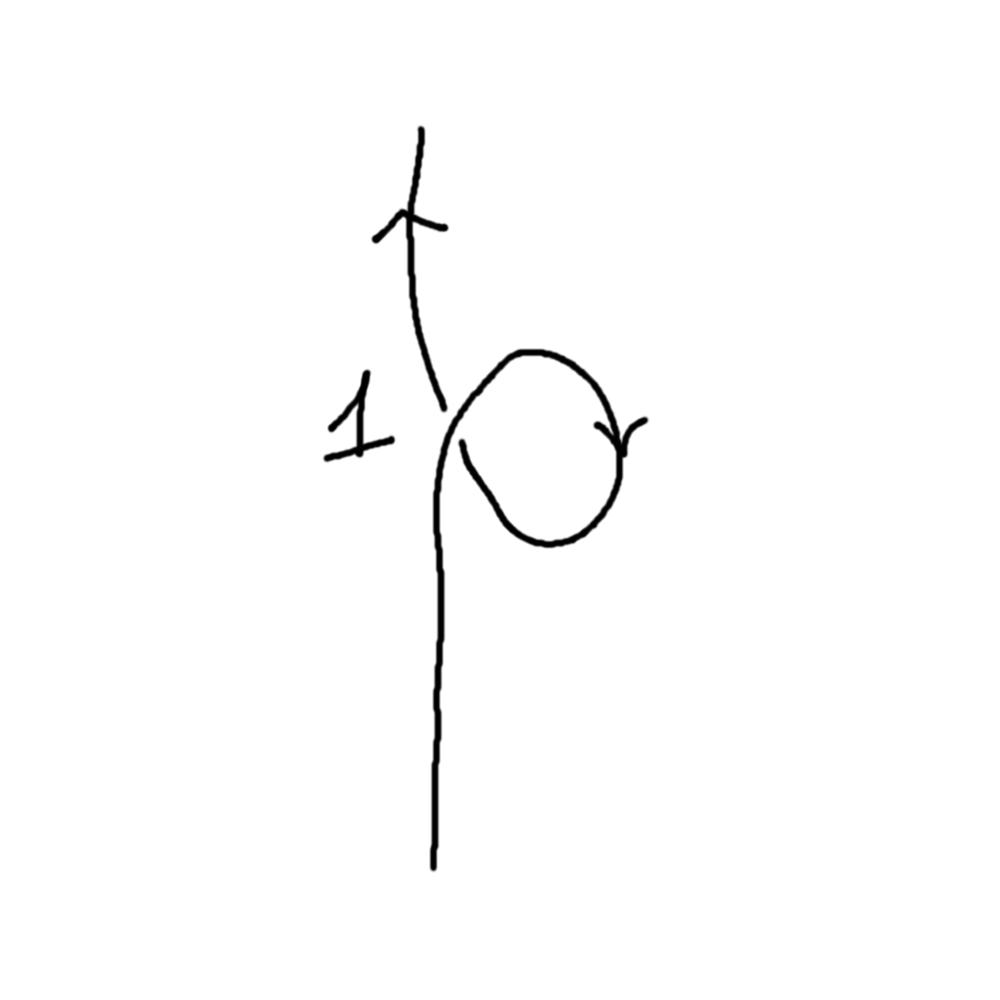
\includegraphics[width=\textwidth]{loop.png}
\caption{$O^{+}_1U^{+}_1$}
\label{fig:loop}
\end{subfigure}
\hfill
\begin{subfigure}{0.31\textwidth}
\centering
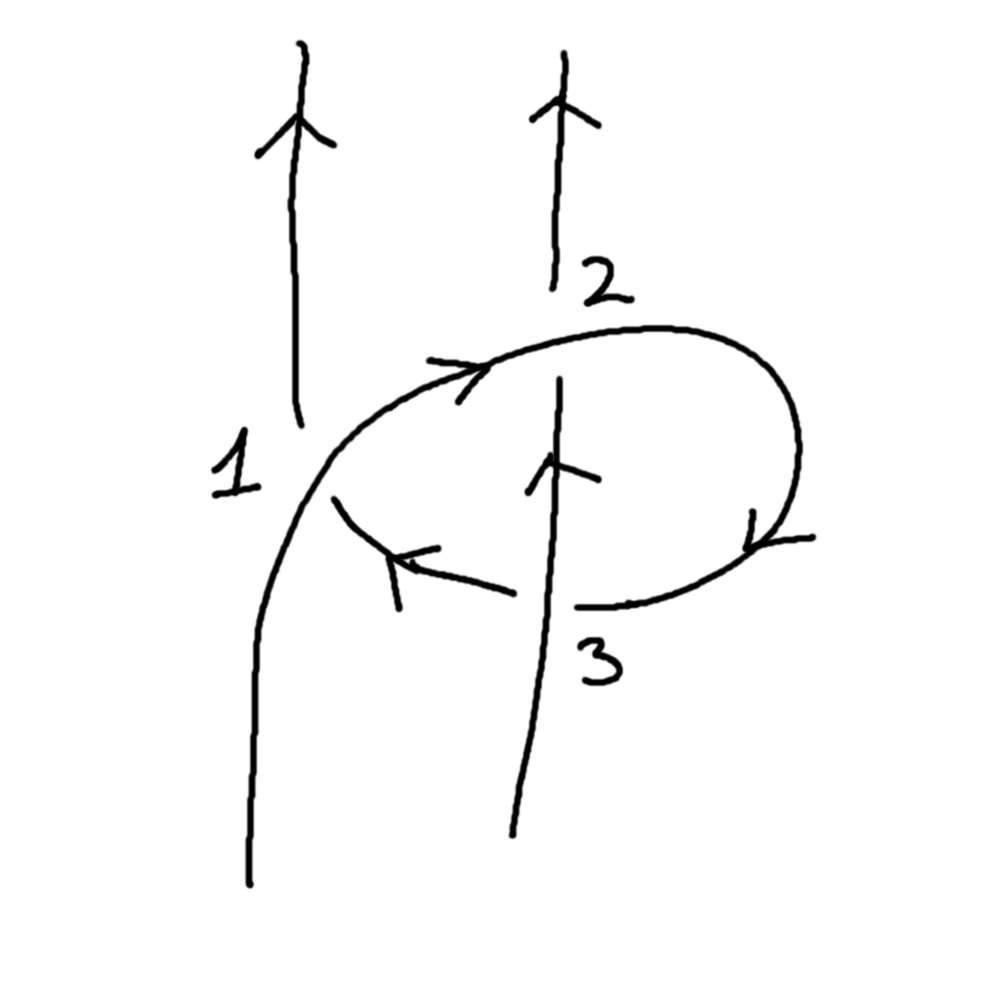
\includegraphics[width=\textwidth]{exampletangle.png}
\caption{$O_1^+O_2^+U_3^+U_1^+,O_3^+U_2^+$ where the left strand is first}
\label{fig:exampletangle}
\end{subfigure}
\hfill
\begin{subfigure}{0.31\textwidth}
\centering
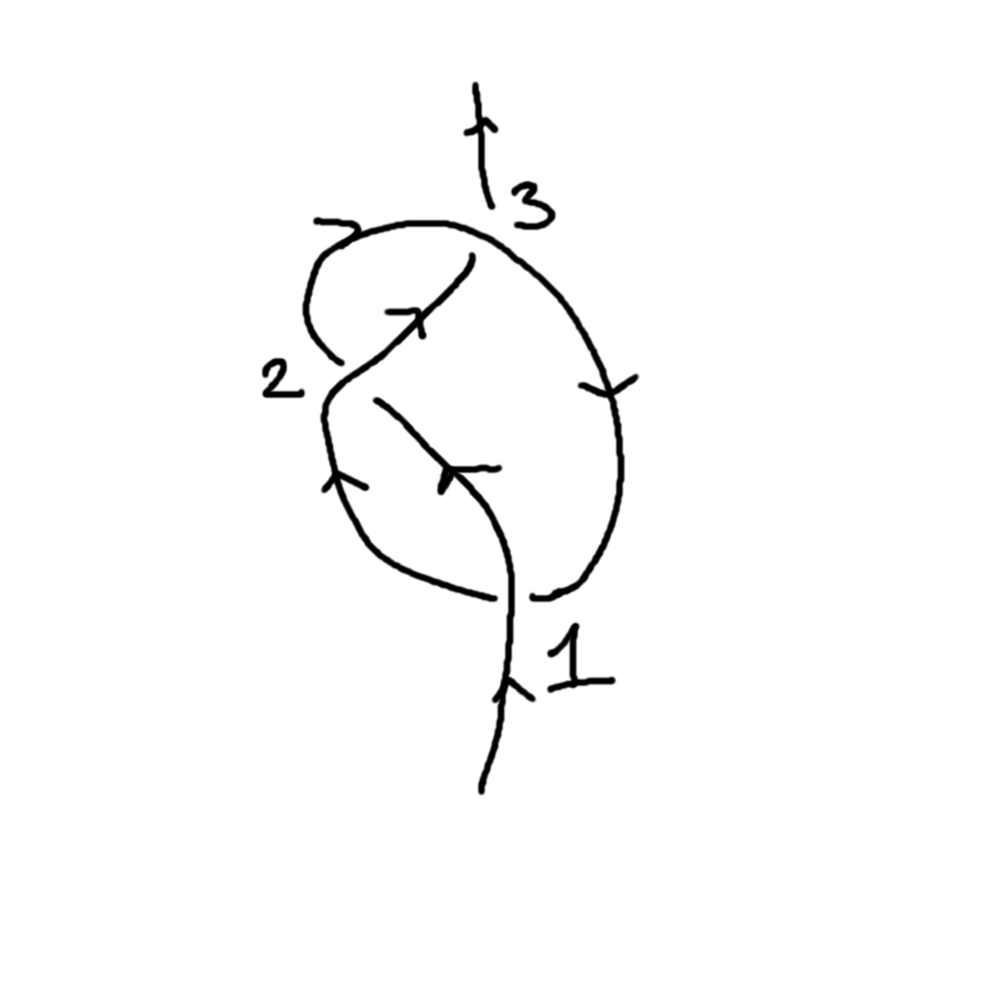
\includegraphics[width=\textwidth]{trefexample.png}
\caption{$O_1^+U_2^+O_3^+U_1^+O_2^+U_3^+$}
\label{fig:trefexample}
\end{subfigure}
\caption{Some examples of Oriented Gauss codes}
\label{fig:Gaussexamples}
\end{figure}

With the Oriented Gauss code we can now define an OU tangle diagram.

\begin{definition}
An OU tangle diagram is a tangle diagram with an Oriented Gauss code, the strings of which can be split in two substrings where the first consists of all $O$s and the second consists of $U$s
\end{definition}

We find an example of an OU tangle diagram in \Cref{fig:exampletangle}, the first string can be split into the substrings $O_1^+O_2^+$ and $U_3^+U_1^+$, the second string can be split into substrings $O_3^+$ and $U_2^+$, hence the diagram is indeed OU. Likewise \Cref{fig:loop} is also an OU tangle diagram, however \Cref{fig:trefexample} is not, since the $O$s and $U$s are mixed together.
				
\section{Reiteration: OU tangle diagrams}

Now we recall a few important concepts from the article \citep{barnatan2020tangles}, on which we base our approach. We define an operation on tangle diagrams, an algorithm, and mention that for the set of diagrams we consider the algorithm does not produce a final result. Instead the algorithm approaches Wild tangles, later we will attempt to describe these wild tangles.

\subsection{The Glide move}

The Glide move as defined in \citep{barnatan2020tangles} is simply an alias for the composition of an R2 and R3 move. We illustrate the Glide move in \Cref{fig:GR2R3}.

\begin{figure}[h!]
\centering
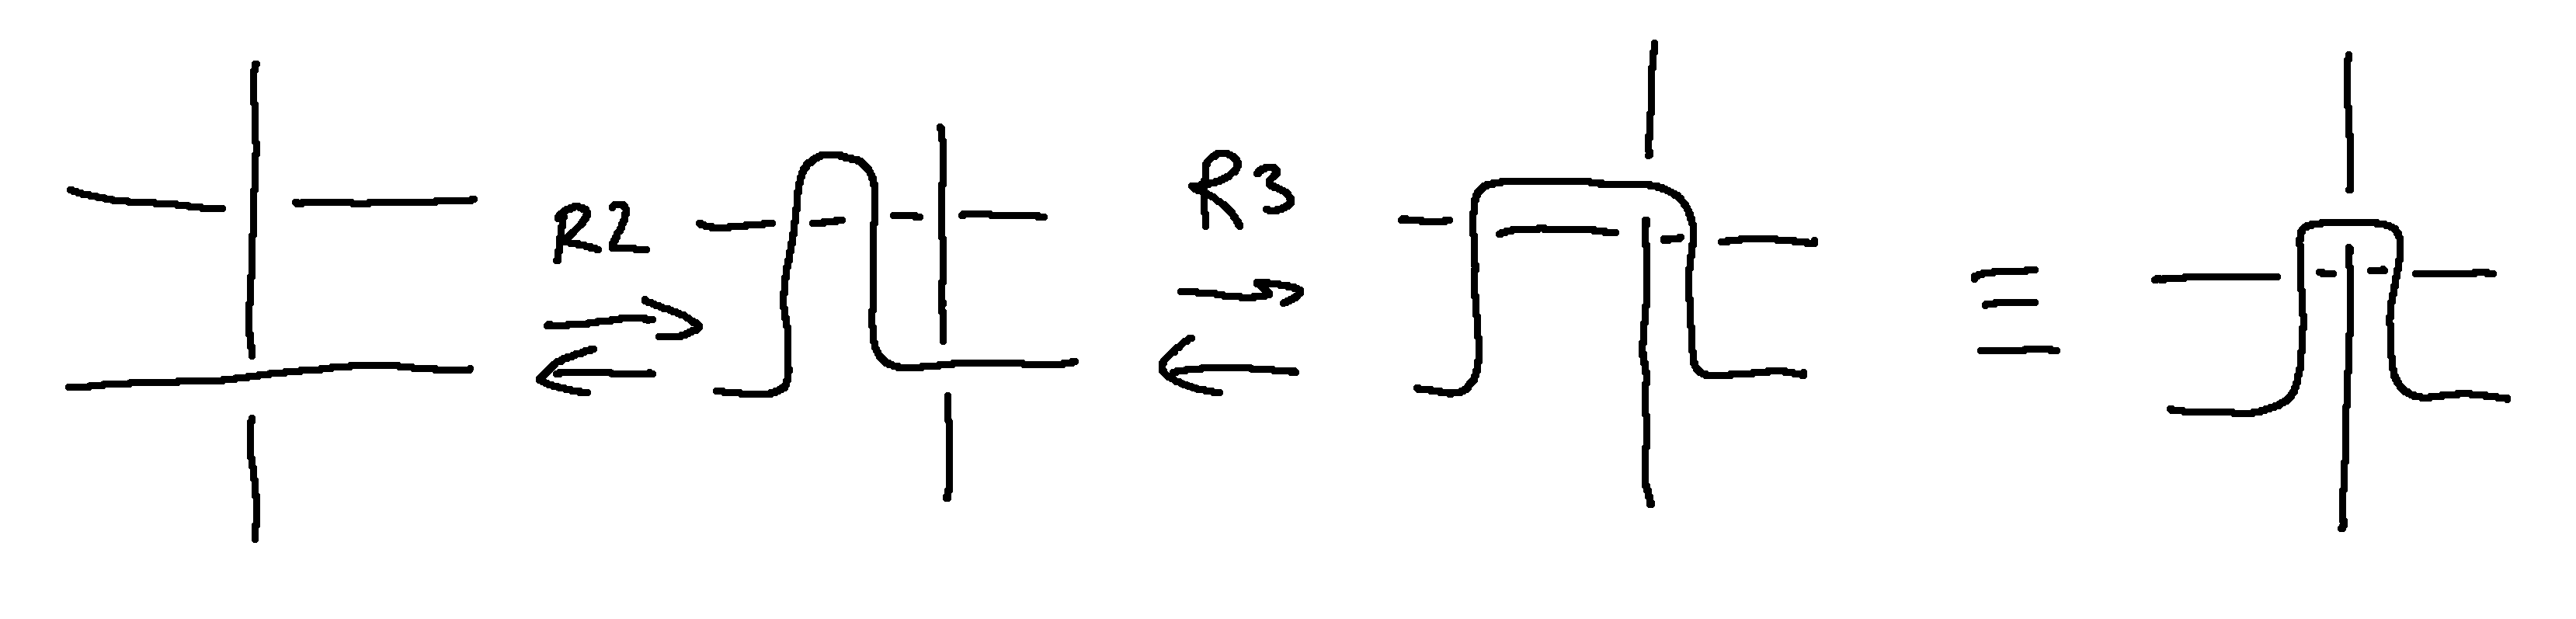
\includegraphics[width=\textwidth]{G=R2+R3.png}
\caption{The Glide move is equivalent to an application of R2 and R3.}
\label{fig:GR2R3}
\end{figure}

The goal of the Glide move is to swap positions of over strands and under strands, i.e. if the Gauss code of a tangle diagram contains $U^s_iO^t_j$ then by a glide move we can swap those symbols to produce a Gauss code with $O^t_iU^s_j$. However this is not the only change the Glide move introduces, other parts of the code are changed since we introduce two new crossings. We can translate the Glide move into an operation on the Oriented Gauss code. This makes it humanly possible to follow the evolution of the diagram upon Gliding. For a tangle diagram with crossings $a,b$ we distinguish 4 cases:
\begin{align*}
U_a^+O_b^-,O_a^+,U_b^-\mapsto O_a^-U_b^+,O_{c}^-O_b^+O_{d}^-,U_{c}^-U_a^-U_{d}^+\\[0.25cm]
U_a^+O_b^+,O_a^+,U_b^+ \mapsto O_a^+U_b^+,O_{c}^+O_b^+O_{d}^+,U_{d}^-U_a^+U_{c}^+\\[0.25cm]
U_a^-O_b^-,O_a^-,U_b^-\mapsto O_a^-U_b^-,O_{d}^+O_b^-O_{c}^+,U_{c}^+U_a^-U_{d}^+\\[0.25cm]
U_a^-O_b^+,O_a^-,U_b^+ \mapsto O_a^+U_b^-,O_{d}^+O_b^-O_{c}^-,U_{d}^+U_a^+U_{c}^-,
\end{align*}
i.e. we replace the substrings of the current Gauss code on the left with their corresponding substrings on the right. We have that $a,b,c,d\in\mathbb N$, the indices $c,d$ can be any number not yet used in the Gauss code. Each case corresponds to a combination of crossing signs, we illustrate the first case in \Cref{fig:glide}.
\begin{figure}[h!]
\centering
\begin{subfigure}{0.40\textwidth}
\centering
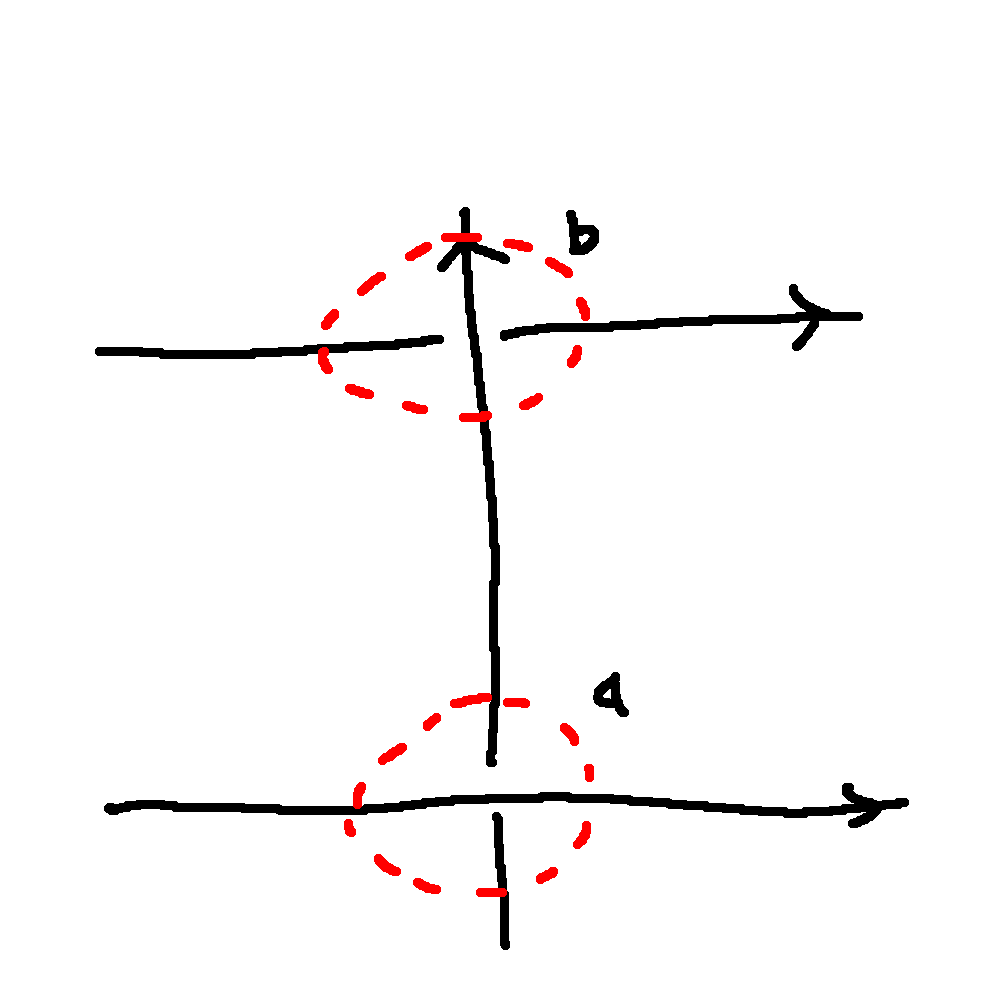
\includegraphics[width=\textwidth]{glide1.png}
\caption{Before applying the Glide move}
\label{fig:glide1}
\end{subfigure}
\hspace{1cm}
\begin{subfigure}{0.40\textwidth}
\centering
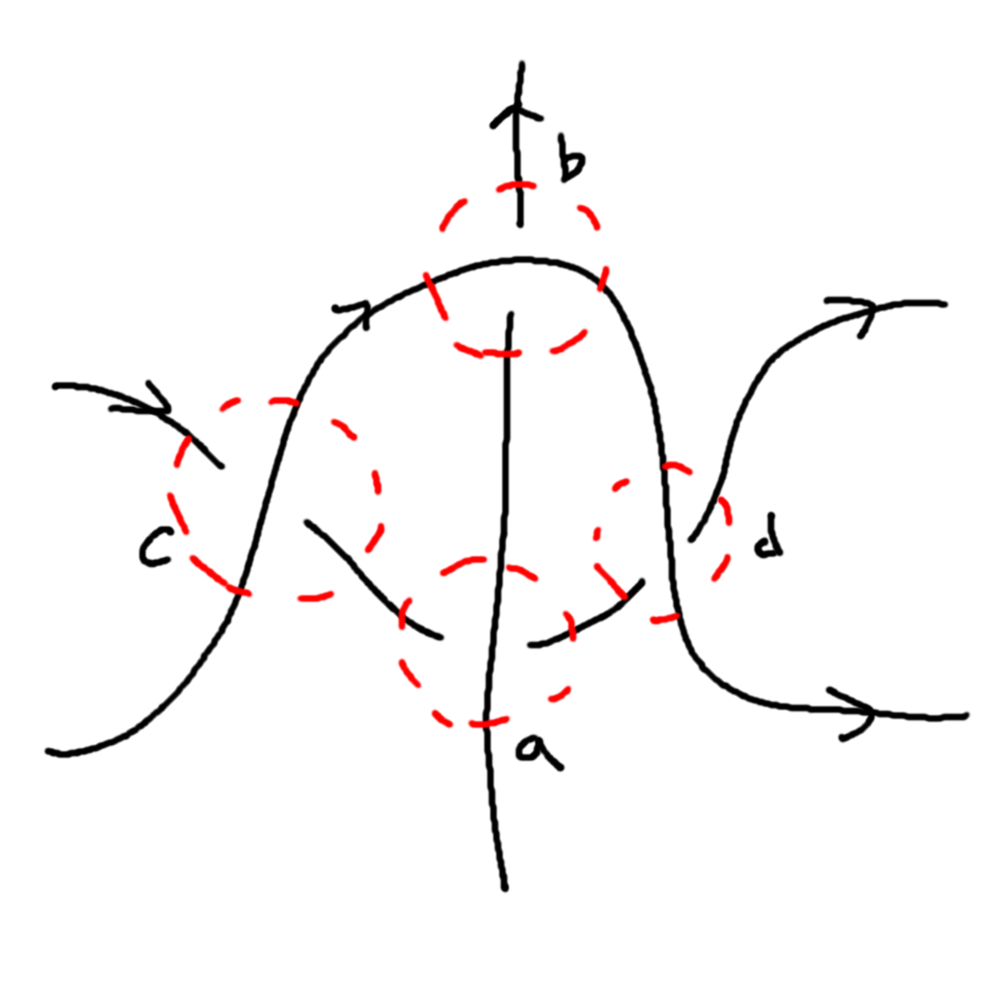
\includegraphics[width=\textwidth]{glide2.png}
\caption{After applying the Glide move}
\label{fig:glide2}
\end{subfigure}
\caption{Example of the Glide move, the triple $U_a^+O_b^-,O_a^+,U_b^-$ are each replaced with $O_a^-U_b^+,O_{c}^-O_b^+O_{d}^-,U_{c}^-U_a^-U_{d}^+$}
\label{fig:glide}
\end{figure}

\subsection{OU Algorithm}
We are now in the position to describe the algorithm from the paper:
\begin{enumerate}
\item For each string in order of occurrence in the Gauss code of the tangle, check each pair of consecutive symbols 
\item If we encounter a pair $U^s_iO^t_j$, apply the Glide move,
\item Simplify the diagram by R1 and R2 moves,
\item If the diagram is in an OU form, we are done, if not return to step 1.
\end{enumerate}

We will proceed in the same way except we will skip step 3. We are more interested in the patterns that arise from iterations of the Glide move, step 3 removes R1 and R2 ``artifacts" in a mostly arbitrary way, in a way we cannot easily follow. Not reducing by R1 and R2 moves should make it simpler to conjecture statements.

For a tangle diagram $D$ we write $\Gamma(D)$ to represent the diagram resulting from the application of the OU Algorithm on $D$. We would hope to see that for each diagram $D$ there exists a $\Gamma(D)$, however it is shown in Theorem 2.3 of \citep{barnatan2020tangles}  that $\Gamma(D)$ only exists for diagrams that are \textit{acyclic}.  

\subsection{Acyclic Diagrams}

\begin{definition}\textbf{(Cyclic Tangle Diagrams)}
A ``cascade path" is a path on the tangle diagram that begins on one of the strands, follows the orientation of the strand it is on, and at a crossing may drop from the upper strand to the lower strand, if desired. A \textit{closed} cascade path is one that returns to its starting position. A diagram is \textit{cyclic} if there exists a closed cascade path, a diagram that is not cyclic is called \textit{acyclic}. 
\end{definition}

An example of an acyclic diagram is given in \Cref{fig:exampletangle} and a cyclic diagram in \Cref{fig:trefexample}. The diagram in \Cref{fig:exampletangle} contains paths that return to the same crossing, however none of them are cyclic since to close the path it is required to jump from an under strand to an over strand. Conversely, on \Cref{fig:trefexample} we have a cycle by:
\begin{enumerate}
\item start on the over strand of crossing 3,
\item follow the orientation through crossing 1,
\item at crossing 2 we are on the over strand, and we choose to jump to the under strand,
\item following the under strand of 2, we arrive at the over strand of 3, where we started.
\end{enumerate}

So we have a criteria for when the OU algorithm terminates for a given tangle diagram. For the case of 1-tangle diagrams we can deduce some information about OU forms before invoking the acyclic property.

\begin{theorem}
All OU tangle diagrams of 1 strand are equivalent by Reidermeister moves to the trivial tangle diagram.
\end{theorem}

\begin{proof}
Consider an OU tangle diagram of 1 strand. Since it is OU, we can split the strand into two parts, one which consists of all over strands, and one with all under strands. Having split the strand into two parts, we notice that the parts are independent of one another, i.e. since the pieces are either all over or all under, they have no interconnections or flips due to crossings. Finally, we can reshape each piece independently to form a straight line, and in the process remove all the crossings. Hence we have a trivial tangle.
\end{proof}

\subsection{Retrospect and further considerations}

So if we encounter an OU 1-tangle diagram, there is nothing much to discuss, the distinction is not useful, since trivial tangle diagrams form only a small proportion of all tangle diagrams. The converse of the statement is not true however, a trivial tangle diagram can also be non OU, simply consider the tangle containing a single Reidermeister 1 move (refer to \Cref{fig:R1move} the bottom  diagram with UO), and here the cyclic property helps distinguish these cases. 

We had made the decision to not reduce by R1 and R2 moves, however this produces issues with the original implementation of the Glide move, specifically, there is a family of tangle diagrams for which the Glide move is not well defined. For example in \Cref{fig:pathology} the OU algorithm will not successfully make a glide move, since the move tries to swap the crossing with itself. As we push the crossing along the under strand, the over strand retreats equally, in such a way we simply circle around indefinitely. Any diagram that contains an R1 move like this will have issues under the OU algorithm, so we decide to ignore crossings like this in step 2 of the algorithm This then implies that in some cases the algorithm can terminate erroneously, which is not a serious problem, since we can simply remove the R1 loop with no issues afterwards.

\begin{figure}
\centering
\begin{subfigure}{0.49\textwidth}
\centering
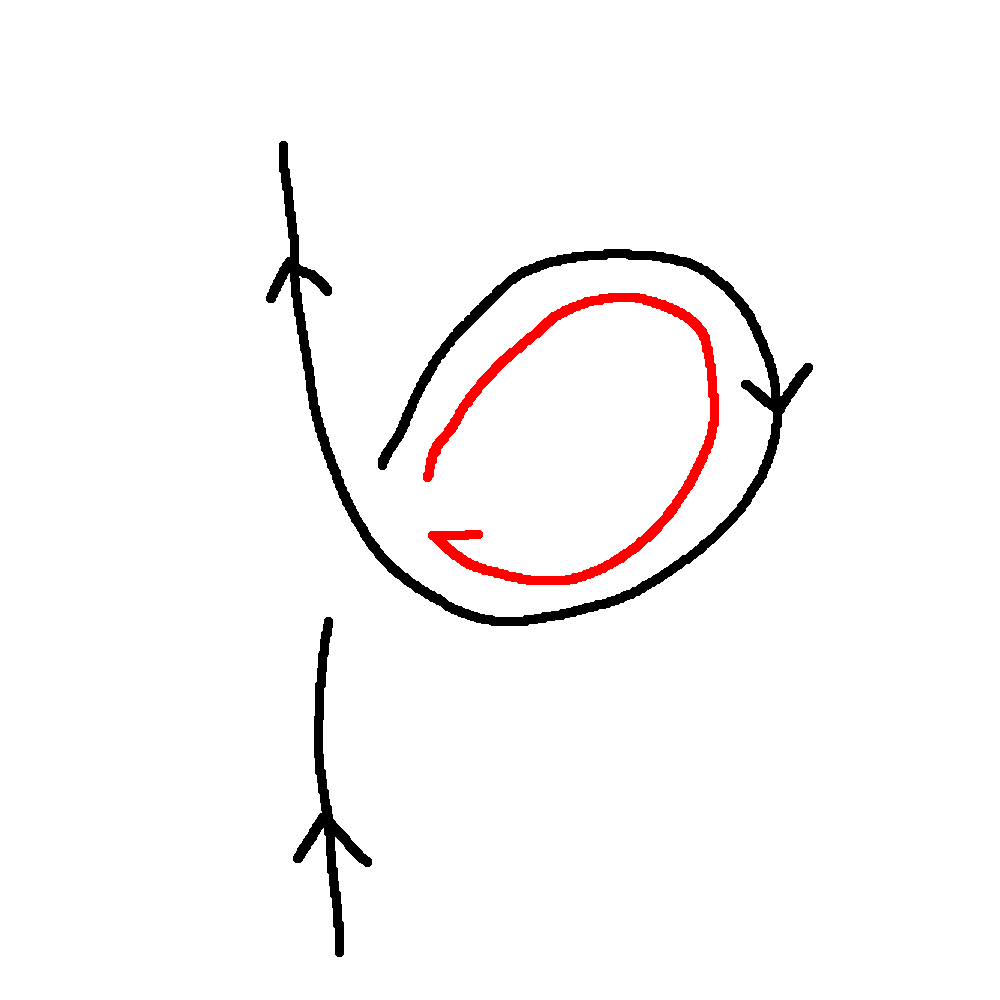
\includegraphics[width=0.7\textwidth]{path1.png}
\end{subfigure}
\hfill
\begin{subfigure}{0.49\textwidth}
\centering
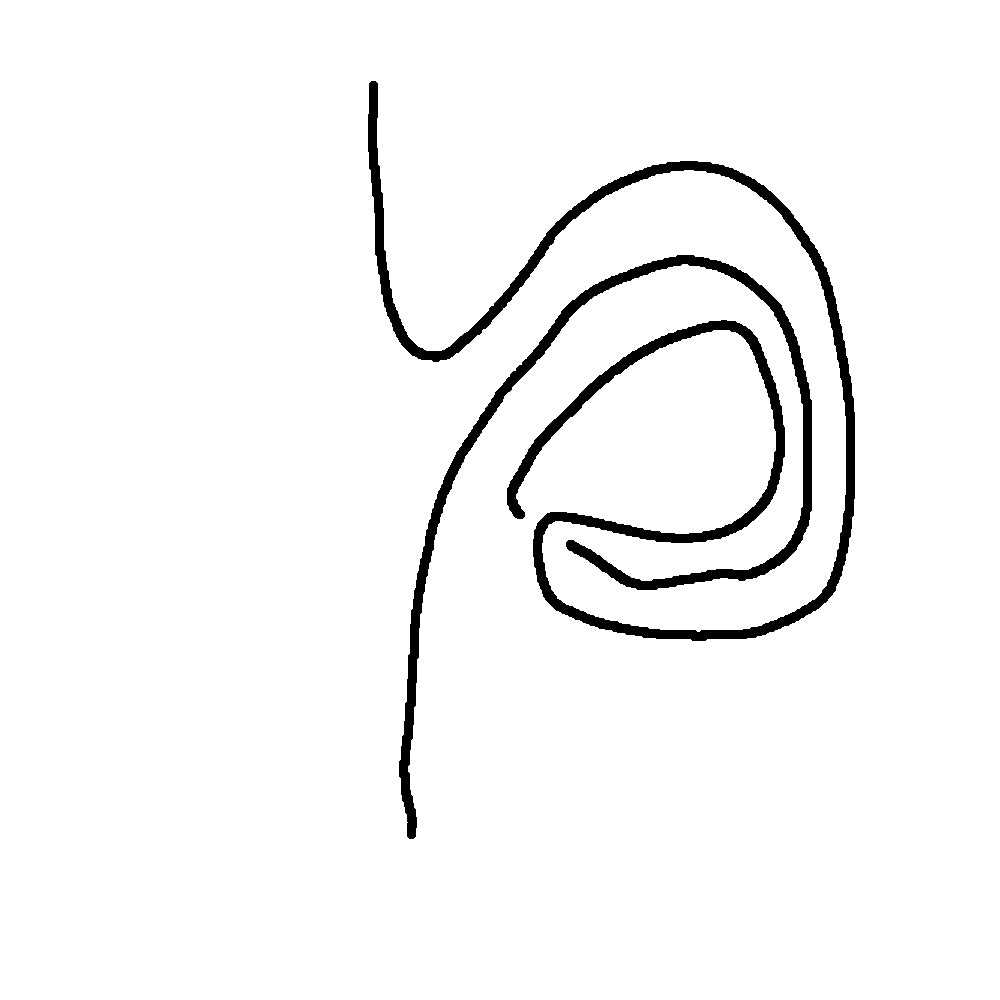
\includegraphics[width=0.7\textwidth]{path2.png}
\end{subfigure}
\caption{A very troublesome tangle}
\label{fig:pathology}
\end{figure}	
\section{The ``Scanning" tangle Drawing Algorithm}

We present a 1-tangle drawing algorithm and a proof of its validity. We call it the ``Scanning" tangle drawing algorithm because one can picture it as a process similar to a braiding board but upside down. The pieces of our finished diagram are attached to the braiding board, and we hold a set containing crossings that we still need to attach. We ``scan" the diagram already on the braiding board and try to find a crossing that we can attach. The scanning must be precise and greedy, otherwise the method is not guaranteed to work. The generic steps of the algorithm can be seen in \Cref{fig:scan}. We now give the algorithm again but more precisely:

% draw each step
\begin{enumerate}
\item Label each segment between the crossings of the tangle. Consider the set of crossings with each end labeled according to the respective connections in the tangle. 
\item Take the first crossing that we encounter along the tangle, leave the end from which we came and attach the three other ends to the scanning front.
\begin{figure}[!h]
\centering
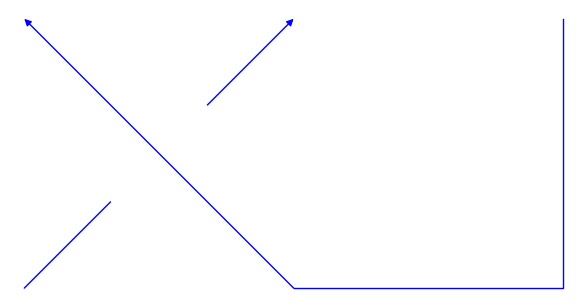
\includegraphics[width=0.4\textwidth]{scanning_0.png}
\caption{The first crossing, the left incoming strand we leave be, the right incoming strand we raise to the ``scanning" front.}
\end{figure}
\item At each iteration read the labels of pairs of ends attached to the front from left to right, and attempt one of the following
\begin{enumerate}
\item If possible attach a new crossing to the two strands, if there exists an unused crossing with those labels (we allow rotating the crossings)
\item If possible attach a new crossing to the left strand, if there exists an unused crossing with that label
\item If neither are possible, try to "cap" off the strands, if they have the same label.
\end{enumerate}
If none of this is possible with the pair, consider the next pair given by the right strand of the previous pair and the strand to the right of it. If none of the consecutive pairs work, then try (b) with the right-most strand.
\begin{figure}[h!]
\centering
\begin{subfigure}[t]{0.3\textwidth}
\centering
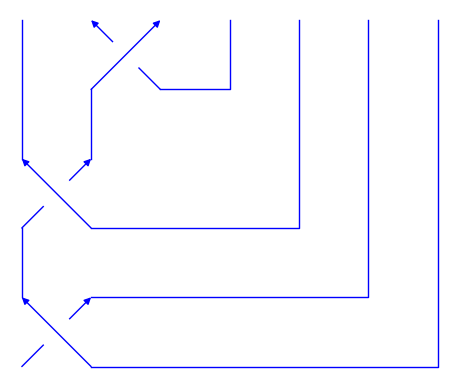
\includegraphics[width=\textwidth]{scanning_2.png}
\caption{Attaching two strands}
\label{fig:scan1}
\end{subfigure}
\hfill
\begin{subfigure}[t]{0.3\textwidth}
\centering
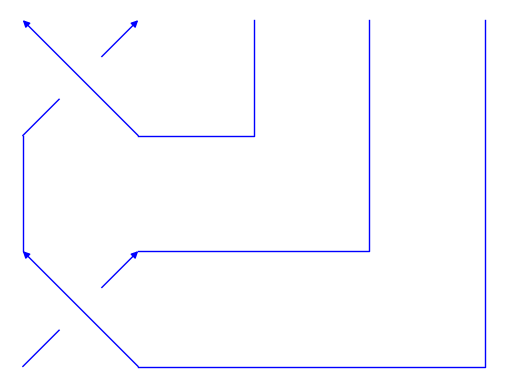
\includegraphics[width=\textwidth]{scanning_1.png}
\caption{Attaching one strand}
\label{fig:scan2}
\end{subfigure}
\hfill
\begin{subfigure}[t]{0.25\textwidth}
\centering
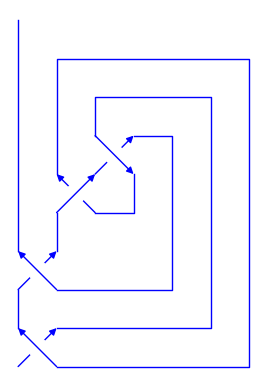
\includegraphics[width=0.8\textwidth]{scanning_3.png}
\caption{Closing a "cap"}
\label{fig:scan3}
\end{subfigure}
\caption{What iterations of the scanning method look like}
\label{fig:scan}
\end{figure}
\item If there is only one strand left on the front, we are done, if there are more, repeat the previous step.
\end{enumerate}

\begin{proof}
What our algorithm essentially does is provide a nice drawing of the tangle diagram, nice in the sense that it aims to not produce extra crossings in the process. It is given that the tangle diagram is planar by definition, so if at every step the diagram with scanning front is planar, then we are guaranteed to have a planar drawing, with no extra crossings.

We see that at the first step, when we fix the first crossing, the diagram is planar. Suppose at some iteration of the algorithm we have a planar diagram, then by affixing a crossing or capping off two strands we do not change the planarity of the diagram. Hence once the algorithm terminates, we have a planar tangle diagram.
\end{proof}


				
\section{Incidence matrices}

Tangle diagrams essentially represent a combination of connections, i.e. strands connect crossings, like edges connect vertices on a graph. Given this similarity, we can construct incidence matrices for the crossings of our tangle diagrams. 

We construct an incidence matrix for a tangle diagram as follows:

\begin{enumerate}
\item Enumerate crossings in order of occurence in the tangle, if we have encountered a crossing before, we skip it. Prepare an ``empty" square matrix $A\in M(n,\{R,G,B,W\})$ where $n$ is the number of crossings, and $R,G,B,W$ represent red, green, blue, and white.
\item For each crossing $i$ in the order, making note of the orientation, we fill entries of $A$ with
\begin{itemize}
\item $A_{ji}=R$
\item $A_{ii}=G$
\item $A_{ki}=B$
\item for all $m\not\in\{i,j,k\}$, $A_{mi}=W$, 
\end{itemize}
where $j,k$ are the crossings left of and right of the crossing $i$ with respect to the over strand, refer to \Cref{fig:incidence} for details
\end{enumerate}

\begin{figure}[h!]
\centering
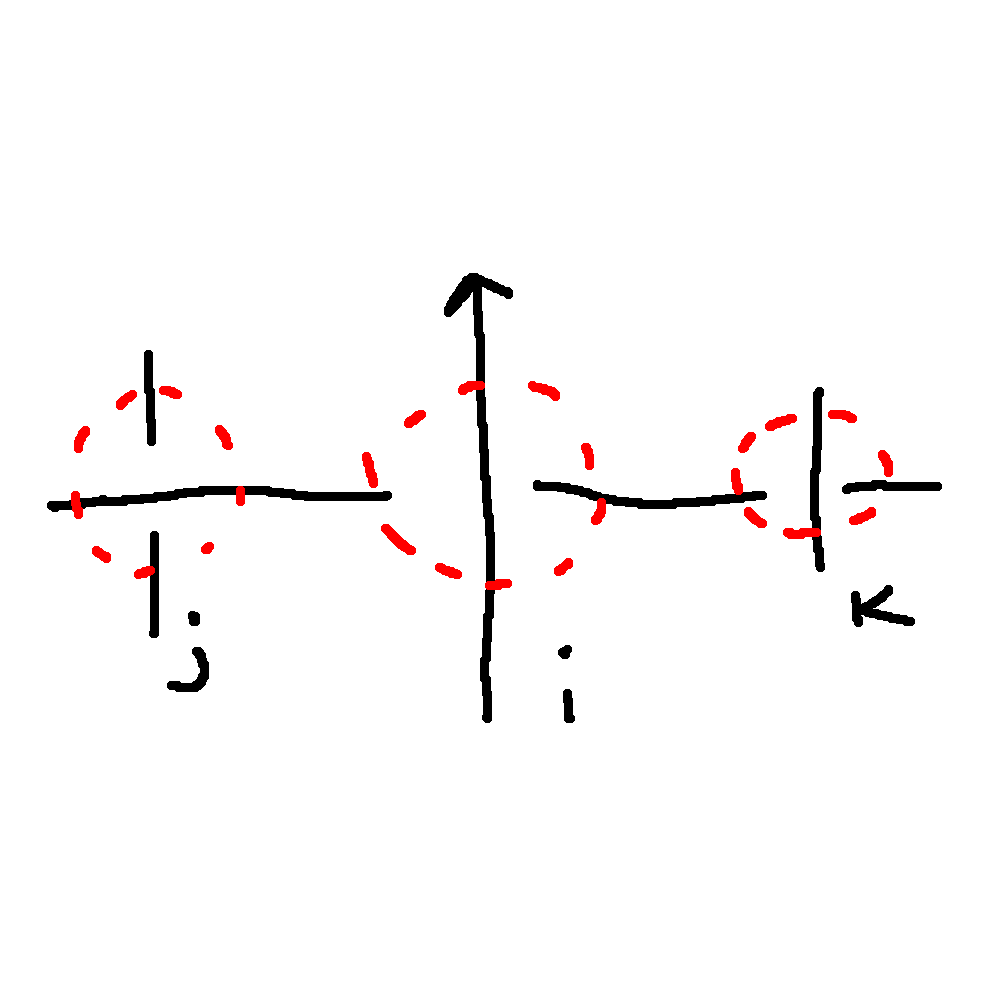
\includegraphics[width=0.4\textwidth]{incidence.png}
\caption{Following the orientation of the crossing $i$, with respect to the over strand, the left crossing is $j$ and the right crossing is $k$. The orientation of the crossings $j,k$ is not important.}
\label{fig:incidence}
\end{figure}

So in other words, each column represents a crossing, and we only consider what is on either side of the crossing. Reading the columns from left to right we get a sense of what crossings are hit. We picked $R,G,B,W$ symbolically, since we wish to plot the matrices, and after a few iterations, any numerical symbols will be illegible. 

We plot some incidence matrices of tangles diagrams corresponding to closed knots from the Rolfsen knot table as found in \citep{rolfsen}. We see interesting patterns emerge! In \Cref{fig:trefR1examples} we have a few instances of the trefoil tangle diagram with an R1 loop added between some crossings, we see that there is some variation after a number of iterations. This variation does not seem to be consistent since the two lower examples have nearly the same incidence matrices, however the first example differs greatly, e.g. the side bands are closer to the diagonal, and the pattern around the diagonal is different.

In \Cref{fig:varioustangleexamples} we have a few more examples but of different tangles. We see similar kind of behavior that as before, some have similar structures, for example, the trefoil and 4,1 have about the same arrangement of squares, the bands and off diagonal patterns, except the colors change. However if we compare them with 9,10 and 10,23, we see variation in features between those two examples, and the previous trefoil and 4,1.

We see distinct and recognisable structures, yet it is not clear what the mechanism behind their production could be.

\newpage

\begin{figure}[H]
\centering
\begin{subfigure}[t]{0.48\textwidth}
\centering
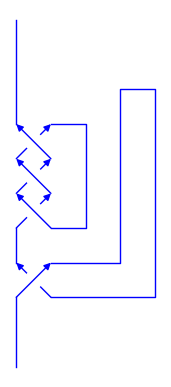
\includegraphics[width=0.30\textwidth]{3_1_ed_0.png}
\end{subfigure}
\hfill
\begin{subfigure}[t]{0.48\textwidth}
\centering
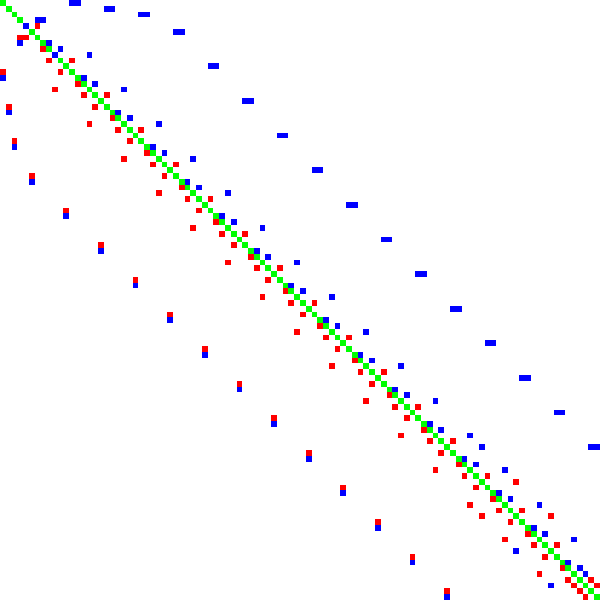
\includegraphics[width=0.8\textwidth]{3_1_R1at0_50.png}
\end{subfigure}
\hfill
\begin{subfigure}[t]{0.48\textwidth}
\centering
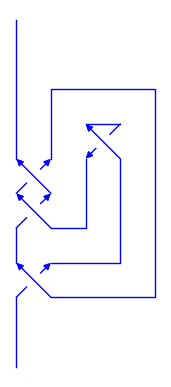
\includegraphics[width=0.3\textwidth]{3_1_ed_2.png}
\end{subfigure}
\hfill
\begin{subfigure}[t]{0.48\textwidth}
\centering
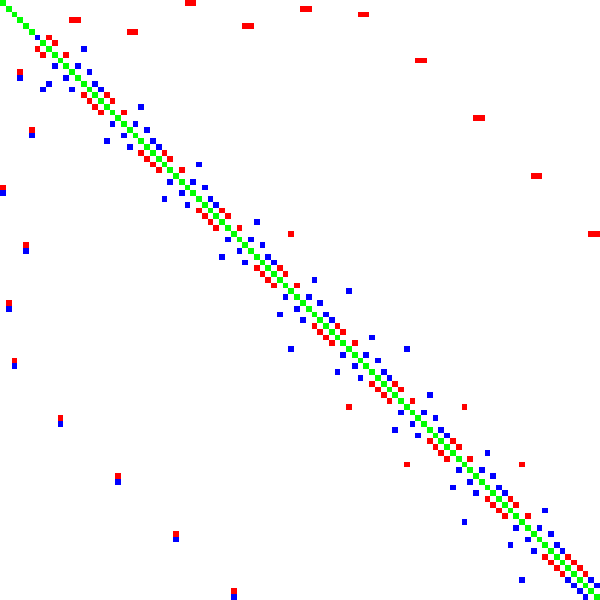
\includegraphics[width=0.8\textwidth]{3_1_R1at2_50.png}
\end{subfigure}
\hfill
\begin{subfigure}[t]{0.48\textwidth}
\centering
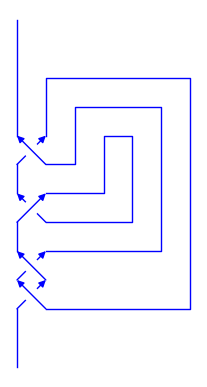
\includegraphics[width=0.3\textwidth]{3_1_ed_4.png}
\end{subfigure}
\hfill
\begin{subfigure}[t]{0.48\textwidth}
\centering
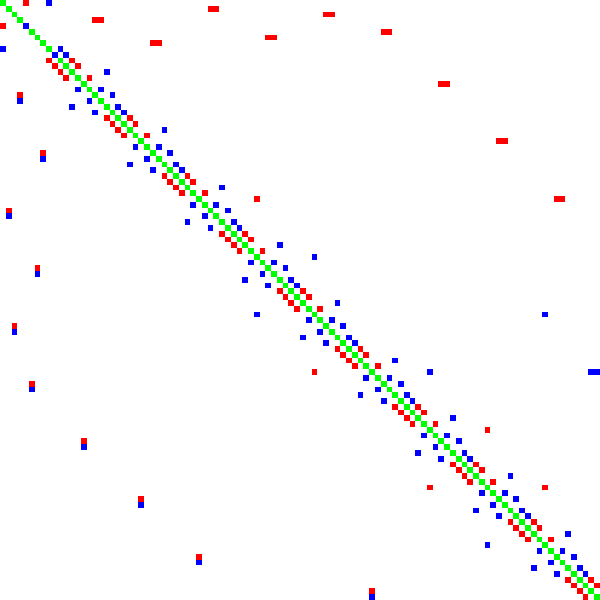
\includegraphics[width=0.8\textwidth]{3_1_R1at4_50.png}
\end{subfigure}
\caption{On the left are diagrams of the trefoil with added R1 loops, on the right their respective incidence matrices after 50 iterations of the OU algorithm}
\label{fig:trefR1examples}
\end{figure}

\begin{figure}[H]
\centering
\begin{subfigure}{0.24\textwidth}
\centering
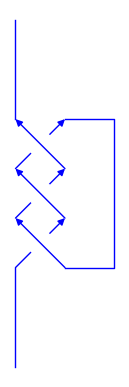
\includegraphics[height=0.25\textheight]{my_trefoil.png} \vfill
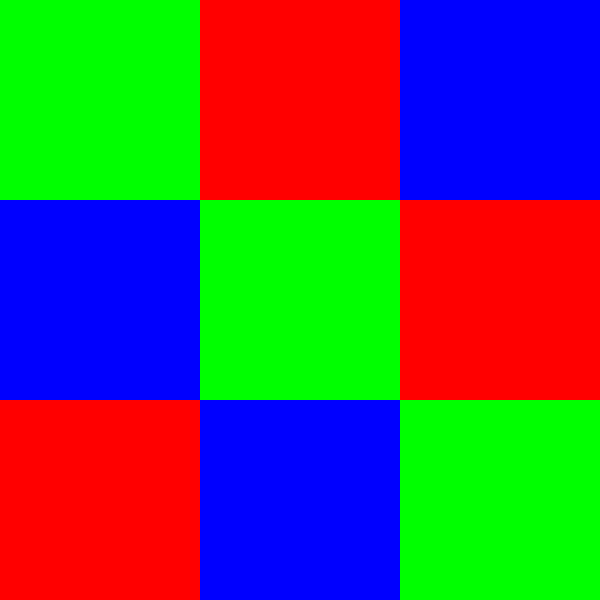
\includegraphics[height=0.15\textheight]{3_1_0.png}       \vfill\vspace{1mm}
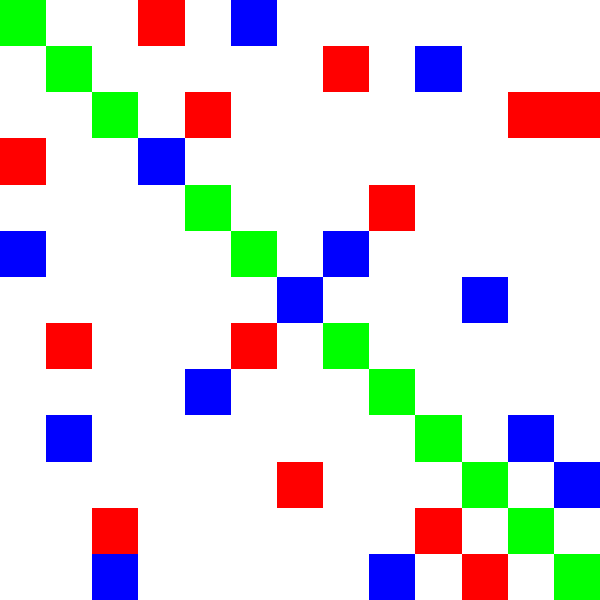
\includegraphics[height=0.15\textheight]{3_1_5.png}       \vfill\vspace{1mm}
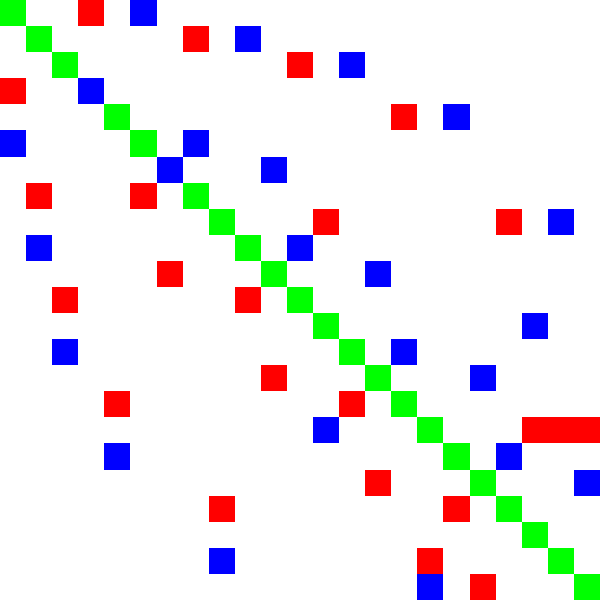
\includegraphics[height=0.15\textheight]{3_1_10.png}      \vfill\vspace{1mm}
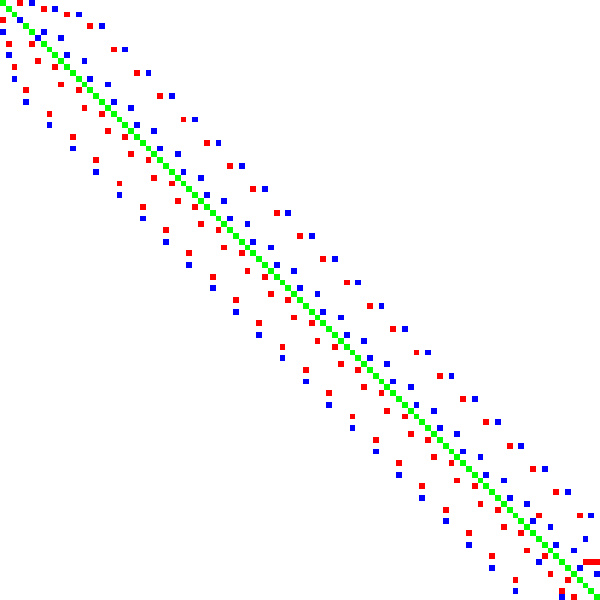
\includegraphics[height=0.15\textheight]{3_1_50.png}
\caption{trefoil diagram}
\end{subfigure}
\hfill
\begin{subfigure}{0.24\textwidth}
\centering
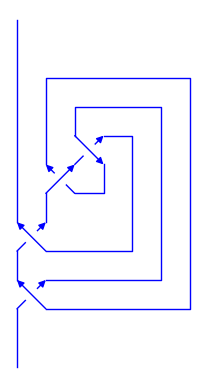
\includegraphics[height=0.25\textheight]{my_4_1.png} \vfill
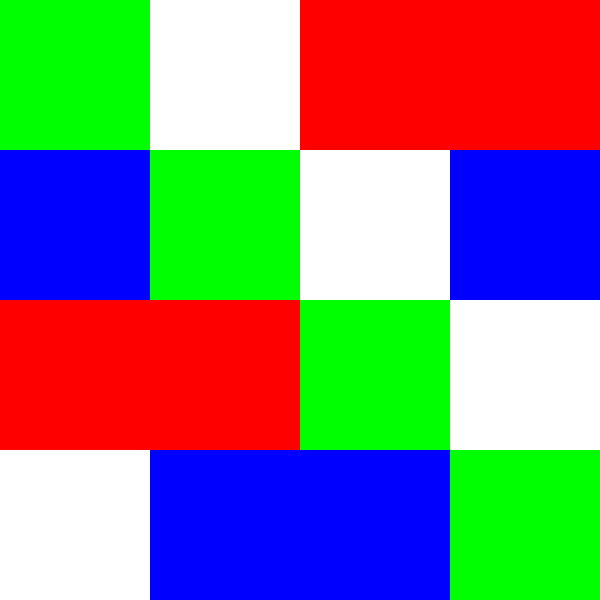
\includegraphics[height=0.15\textheight]{4_1_0.png}  \vfill\vspace{1mm}
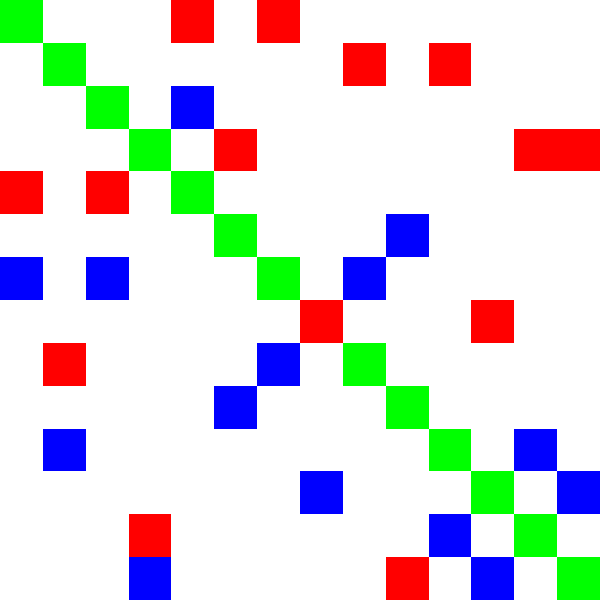
\includegraphics[height=0.15\textheight]{4_1_5.png}  \vfill\vspace{1mm}
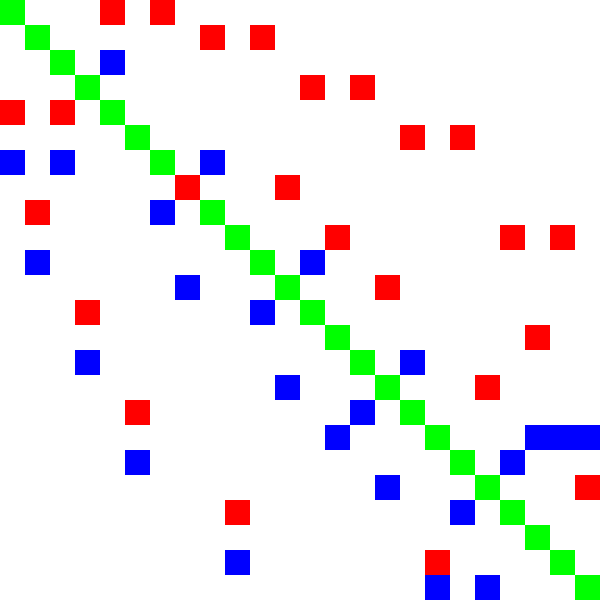
\includegraphics[height=0.15\textheight]{4_1_10.png} \vfill\vspace{1mm}
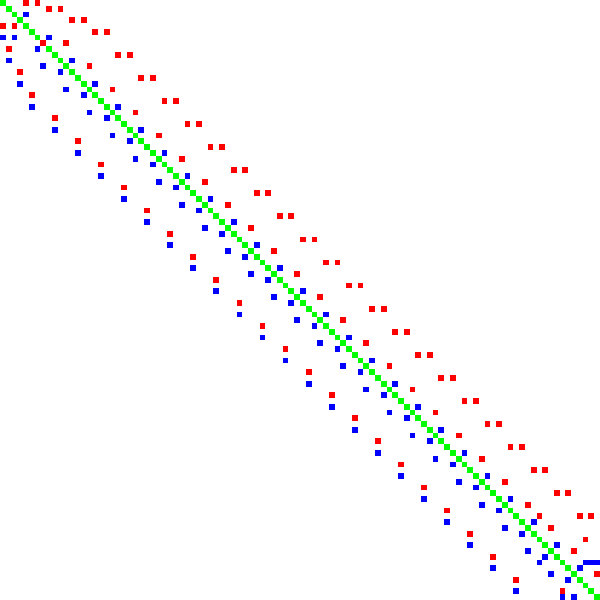
\includegraphics[height=0.15\textheight]{4_1_50.png} \vfill\vspace{1mm}
\caption{4,1 diagram}
\end{subfigure}
\hfill
\begin{subfigure}{0.24\textwidth}
\centering
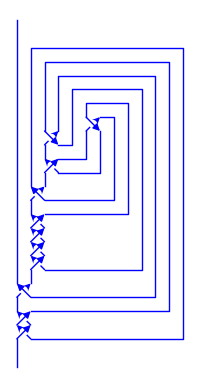
\includegraphics[height=0.25\textheight]{my_9_10.png} \vfill
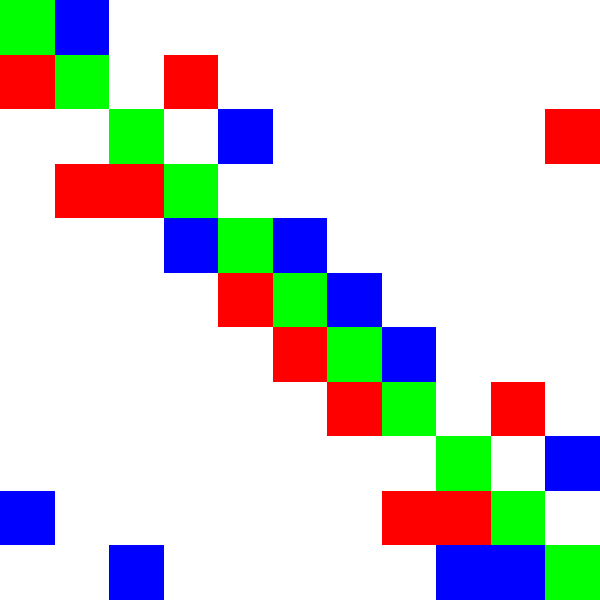
\includegraphics[height=0.15\textheight]{9_10_0.png}  \vfill\vspace{1mm}
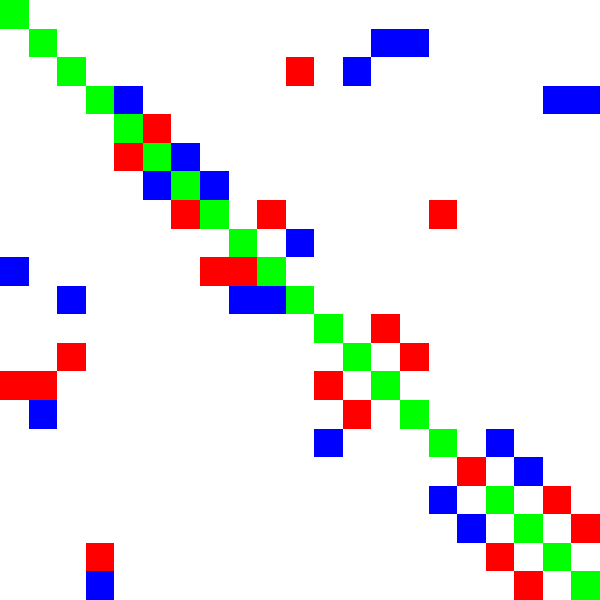
\includegraphics[height=0.15\textheight]{9_10_5.png}  \vfill\vspace{1mm}
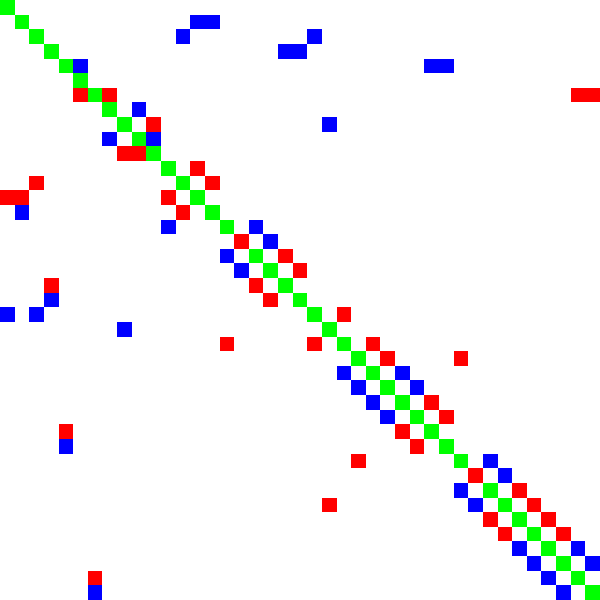
\includegraphics[height=0.15\textheight]{9_10_10.png} \vfill\vspace{1mm}
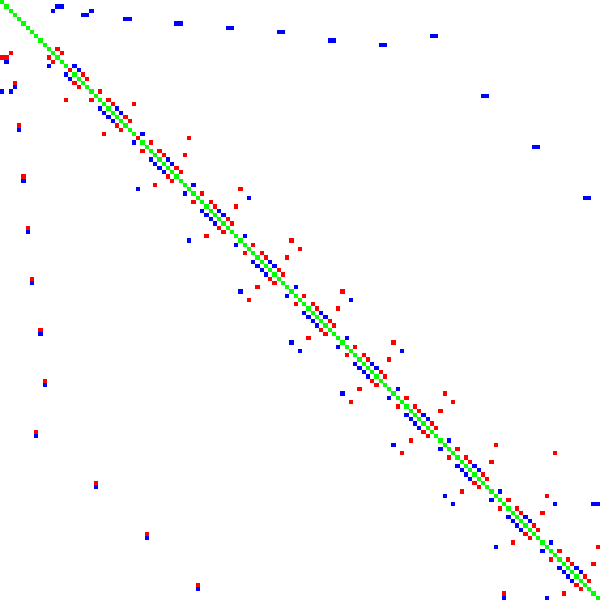
\includegraphics[height=0.15\textheight]{9_10_50.png} \vfill\vspace{1mm}
\caption{9,10 diagram}
\end{subfigure}
\hfill
\begin{subfigure}{0.24\textwidth}
\centering
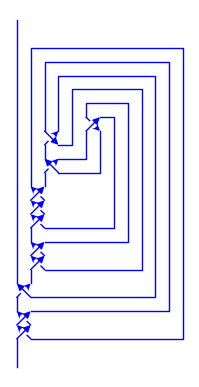
\includegraphics[height=0.25\textheight]{my_10_50.png} \vfill
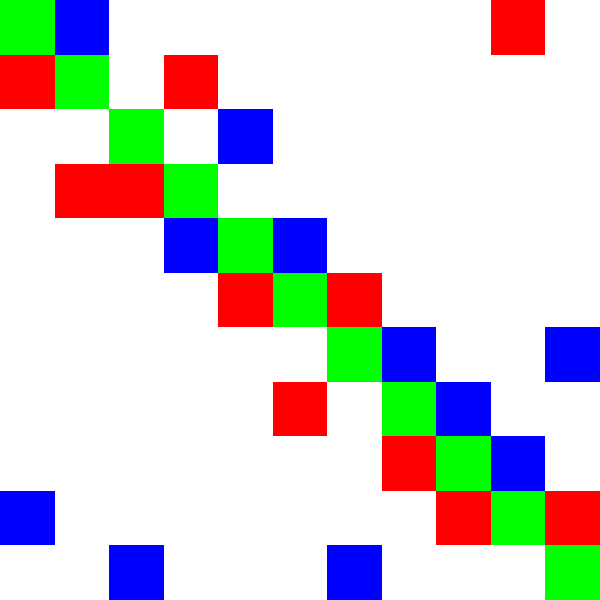
\includegraphics[height=0.15\textheight]{10_50_0.png}  \vfill\vspace{1mm}
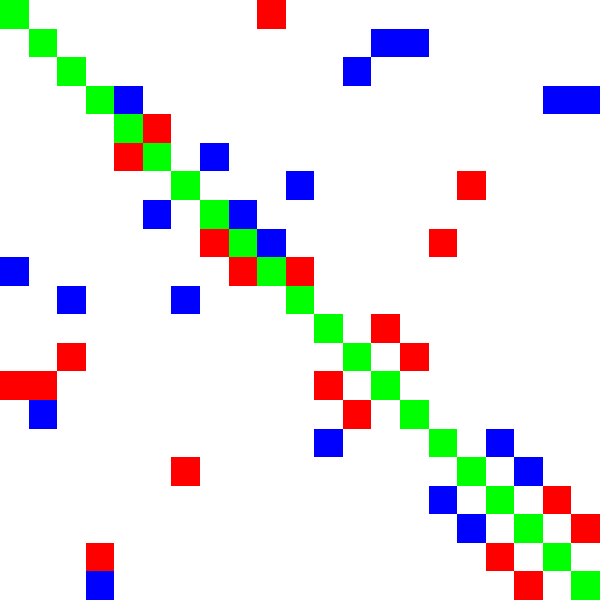
\includegraphics[height=0.15\textheight]{10_50_5.png}  \vfill\vspace{1mm}
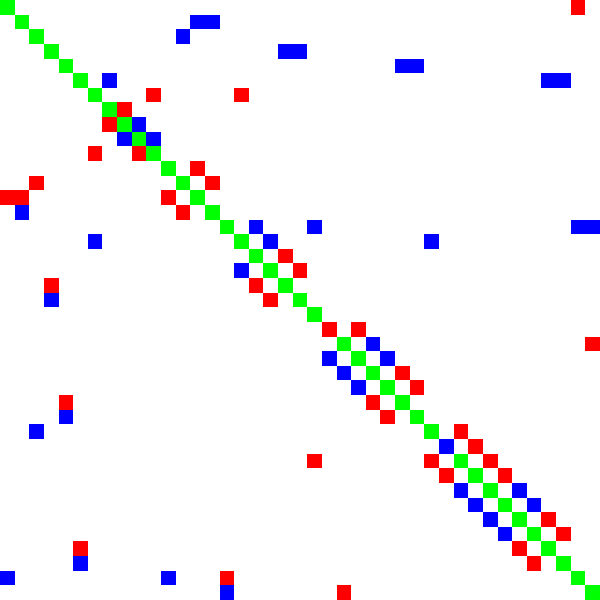
\includegraphics[height=0.15\textheight]{10_50_10.png} \vfill\vspace{1mm}
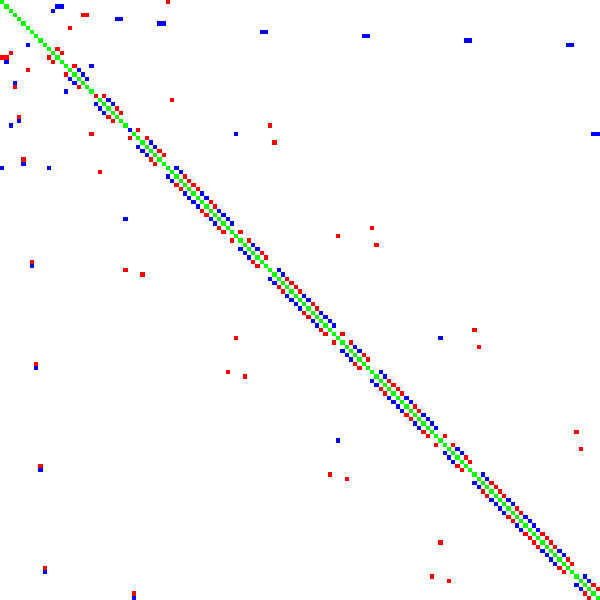
\includegraphics[height=0.15\textheight]{10_50_50.png} \vfill\vspace{1mm}
\caption{10,23 diagram}
\end{subfigure}
\caption{Comparing incidence matrices of several tangles diagrams under the OU algorithm. Each column is a separate tangle, each column is 0, 5, 10, 50 iterations}
\label{fig:varioustangleexamples}
\end{figure}			\newpage
\section{Conclusions and Further work}

\subsection{What we did}

From \Cref{fig:trefR1examples} and \Cref{fig:varioustangleexamples} we see that we indeed produce periodic structures with differences from tangle to tangle, and between different starting tangle diagrams. We did not however conclude how these patterns arise. 

We only considered a few example diagrams for the trefoil tangle, perhaps for different tangles we will see different results. 

Another option is to consider Knots instead of Tangles, so that the glide move may wrap around the starting and end strands. 

\subsection{Convergence}

We mentioned a distinction between tame and wild diagrams, yet never suggested any sort of convergence of tame diagrams to wild ones. As the OU algorithm progresses the incidence matrix grows without bound, in such a way producing an infinite structure. If we consider the sequence of incidence matrices as submatrices of infinite matrices, and pick appropriate values for our symbolic R,G,B,W, we may define convergence, and see if it produces any meaningful results.

\subsection{Code and accumulated data}

For computations and to produce the images (the matrices, and the blue tangle diagrams) we used the \texttt{SageMath} package and its respective Knot Theory module. We export the code after the references. We have precomputed and compiled a large body of data, and stored it in a convenient place \citep{observations}. Specifically, videos in \texttt{.avi} format of sequences of incidence matrices for tangles corresponding to knots in \citep{rolfsen} (we used the Oriented Gauss Code as given by each knot).		\newpage
\bibliography{references.bib}
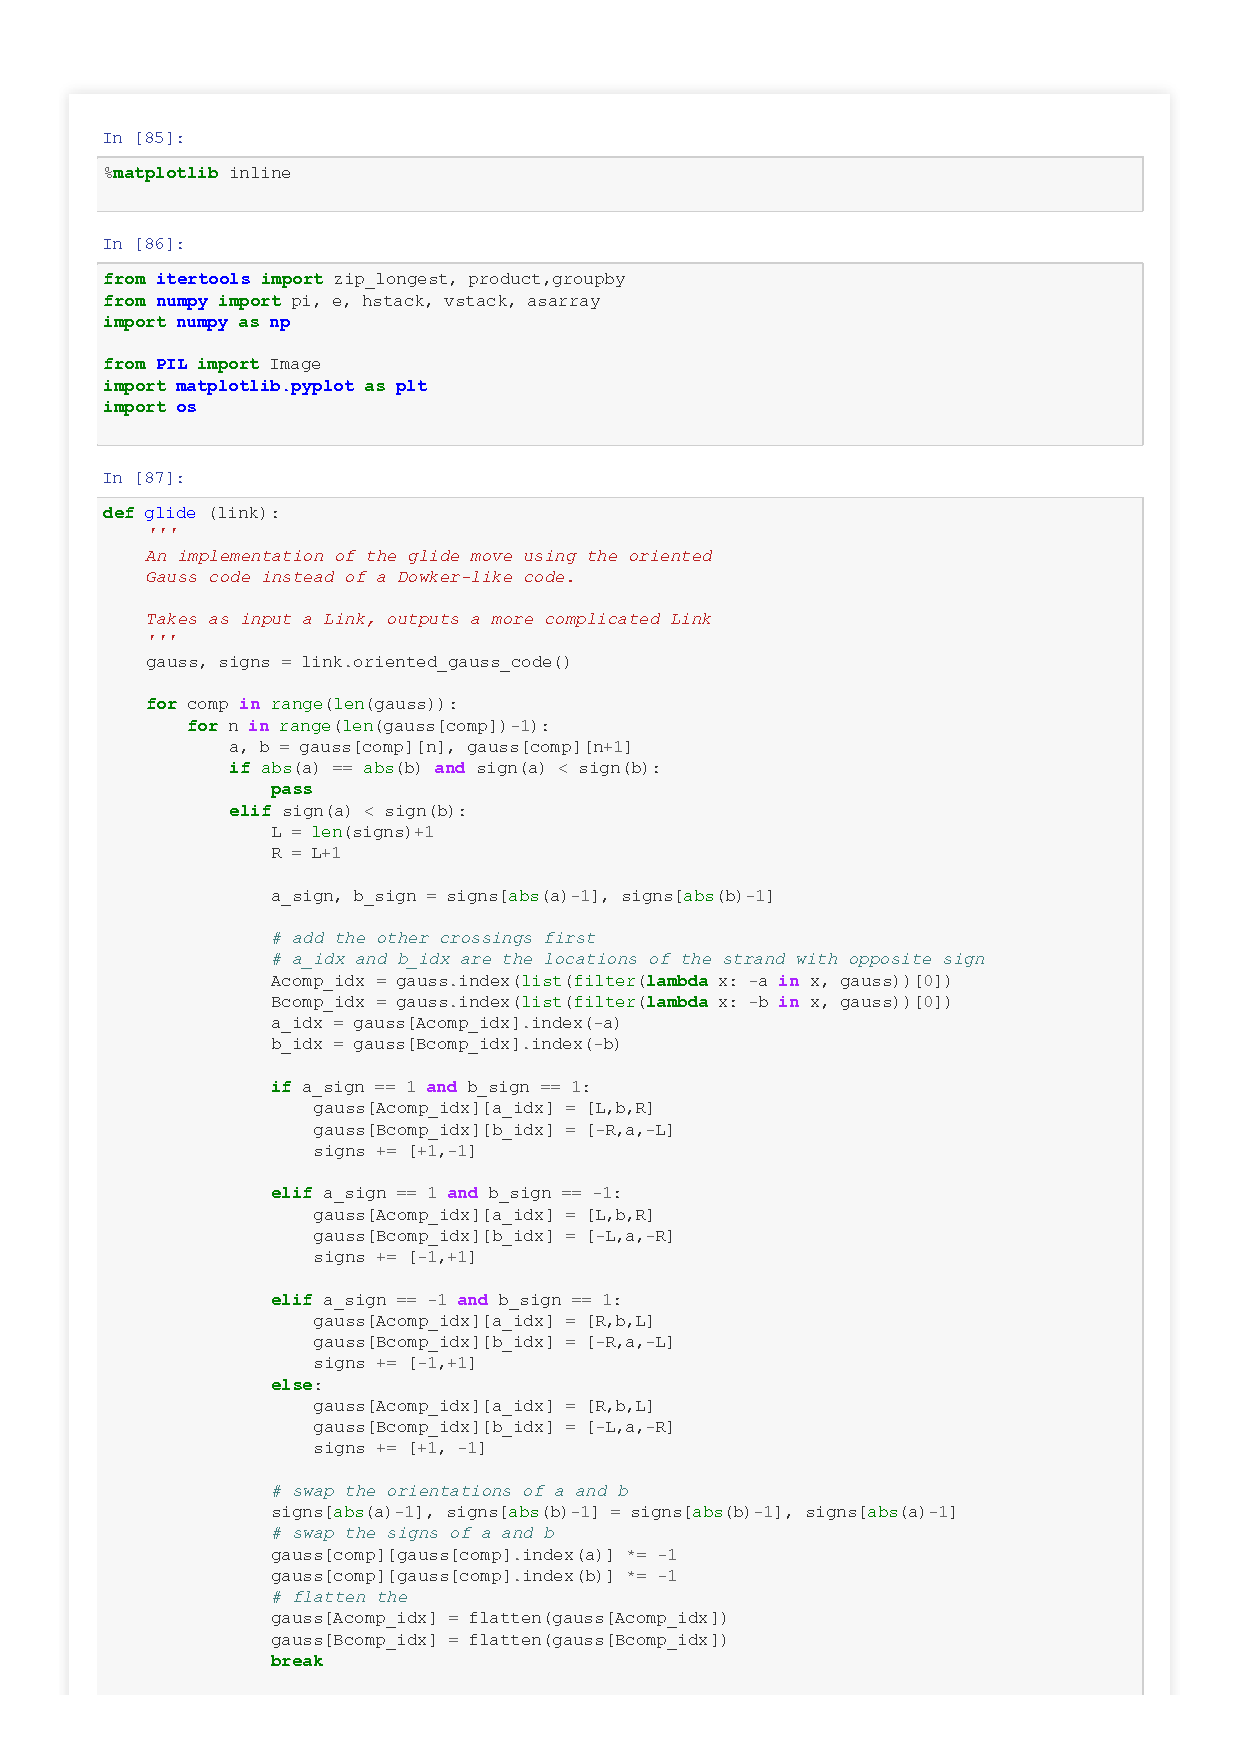
\includepdf[pages=-]{Observations.pdf}

\end{document}